% tm project ignores: !(/\.(?!htaccess)[^/]*|\.(tmproj|o|pyc|toc|aux|xyc|bbl|blg|lof|lot|out|synctex\.gz)|/Icon\r|/svn-commit(\.[2-9])?\.tmp)$

%   Modified   92-09-18      Add references to dissertation        D. Teale
%                            Add approval page to toc
%                            Add ref to Title Degree on approval page
%   Modified  2006-09-12     Added geometry package to set up UofC thesis margins
%                            Removed includeprompt option N. Mancell
%
% Modified  2012-04-15  T.Zhang
% 1, the ``fancy'' package is cancelled. The pagestyle is changed from ``myheadings''
%    and ``headings'' to ``plain'' to move the page number (footer) from top right to bottom centre.
% 2, The parameter  of using ``geometry'' package is changed from four different values
%     (top=1in, bottom=1.22in, left=1.40in, right=0.850in) to one single value:
%     1in (top=1in, bottom= 1in, left= 1in, right= 1in)
% 3, ``List of Figures'' is modified to ``List of Figures and Illustrations''
% 4, A new page ``List of Symbols, Abbreviations and Nomenclature'' is created.
%    Its page number is following ``List of Figures and Illustrations'' with Roman numerals.
%    A separate file ``symbols.tex'' is created for students to put content into the list.





\documentclass{ucalgthes1}
\usepackage[letterpaper,top=1in, bottom= 1in, left= 1in, right= 1in]{geometry}
%\usepackage{fancyhdr}
%\fancyhead{}
%\fancyfoot{}
%\renewcommand{\headrulewidth}{0pt}
%\fancyhead[RO,LE]{\thepage}
%Define other usepackages here

%!TEX root = /Users/gilesb/UofC/thesis/phd-thesis/phd-thesis.tex

%\usepackage[T1]{fontenc}
%\usepackage[utf8]{inputenc}
%\usepackage{palatino,courier}
\usepackage[reqno]{amsmath}
\usepackage{amsthm}
\usepackage{amsfonts,amssymb}
\usepackage{mathrsfs}   % special script style \mathscr{S}
\usepackage[mathscr]{euscript}
\usepackage[all]{xy}
\usepackage{stmaryrd}
\usepackage{graphicx}
\usepackage{array}
\usepackage{fancyvrb}
\usepackage{proof}
%\usepackage{mchaskell}
\usepackage{float}
%\usepackage{makeidx}
%\usepackage{url}
\usepackage{varioref}
%\usepackage{listings}

%\usepackage{mylhs}
\usepackage{wrapfig}
\usepackage{subfig}
\usepackage{caption}
\usepackage{supertabular}
\usepackage{blkarray}

\usepackage{xspace}
\usepackage[colorlinks=true,citecolor=magenta]{hyperref} 
\usepackage{hyperref}
%\usepackage{lqpl}
\usepackage{prettyref}

\usepackage{tikz}
\usetikzlibrary{calc,arrows,positioning}

\reversemarginpar

\captionsetup{style=default,labelfont={bf}}
\def\figurename{Figure}
\def\tablename{Table}

% This causes horrid processing error - text garbage appearing instead of 
% The diagram. DO NOT USE \CompileMatrices


\graphicspath{{./diagrams/}{.}}
%
%include lhs2TeX.fmt
%include lhs2TeX.sty
%format ^* = "\ltimes"
%format *^ = "\rtimes"
% captionskips do not seem to be defined in uc class
\makeatletter
%%\newlength\abovecaptionskip
%%\newlength\belowcaptionskip
\setlength\abovecaptionskip{10\p@}
\setlength\belowcaptionskip{0\p@}
\makeatother

\input{macros-all}
\title{An investigation of the underpinnings of quantum and reversible computing \\
\bigskip subtitle }
%
%            Insert the correct information between the {}
%
\author{Brett Gordon Giles}
\thesisyear{2013}
\thesis{dissertation}    % the word dissertation can be inserted between {}
\newcommand{\thesistitle}{An investigation of the underpinnings of quantum and reversible computing}
\monthname{August}
\dept{COMPUTER SCIENCE}
\degree{DOCTOR OF PHILOSOPHY}
%
%                    End of supplied information
%
\begin{document}
\makethesistitle
\pagenumbering{roman}     % resets page counter to one
\setcounter{page}{1}
%\chapter*{UNIVERSITY OF CALGARY \\ FACULTY OF GRADUATE STUDIES}
%\thispagestyle{empty}
%The undersigned certify that they have read, and recommend
%to the Faculty of Graduate Studies for acceptance, a \Thesis\ entitled
%``\thesistitle'' submitted by \Author\
%in partial fulfillment of the requirements for the degree of
%\Degree.\\

%
%                 Substitute  List of Examiners
%
%\begin{signing}{Department of Academic Computing}
%\signline
%Chairman, Dr.~John D.~Doe \\
%Department of Academic Computing \\
%Services  \\
%\signline
%Chairman, Dr.~John D.~Doe \\
%Department of Academic Computing \\
%Services  \\
%\signline
%Chairman, Dr.~John D.~Doe \\
%Department of Academic Computing \\
%Services  \\
%\signline
%Chairman, Dr.~John D.~Doe \\
%Department of Academic Computing \\
%Services  \\
%\newsigncolumn         use this command to start a new column if necessary
%\newsigncolumn
%\signline
%Chairman, Dr.~John D.~Doe \\
%Department of Academic Computing \\
%Services  \\
%\signline
%Dr.~Jane Smith \\
%Department of Academic Computing  \\

%\signline
%Dr.~A.~B.~Brown \\
%Department of Academic Computing  \\
%\end{signing}
%
\newpage
\phantomsection
\altchapter{\bf{Abstract}}

\newpage
\phantomsection
\altchapter{\bf{Acknowledgements}}


\begin{singlespace}
\newpage
\phantomsection
\tableofcontents
\pagestyle{plain}
\newpage
\phantomsection
\listoftables
\pagestyle{plain}
\newpage
\phantomsection
\listoffigures
\pagestyle{plain}
\clearpage
\clearpage          % otherwise tables will be numbered wrong
\end{singlespace}
\newpage
\phantomsection
\chapter*{\bf{List of Symbols, Abbreviations and Nomenclature}\hfill} \addcontentsline{toc}{chapter}{List of Symbols}
\listofsymbols
%\pagestyle{plain}
%\clearpage


\pagenumbering{arabic}
%!TEX root = /Users/gilesb/UofC/thesis/phd-thesis/phd-thesis.tex

\chapter{Quantum computation}\label{chap:quantum_computation}

\section{Linear algebra} % (fold)
\label{sec:linear_algebra}

Quantum computation requires familiarity with the basics of linear algebra. This section will give
definitions of the terms used throughout this thesis.
\subsection{Basic definitions} % (fold)
\label{sub:basic_definitions}


The first definition needed is that of a \emph{vector space}.

\begin{definition}[Vector Space]
  Given a field $F$, whose elements will be referred to as scalars, a \emph{vector space} over $F$
  is a non-empty set $V$ with two operations, \emph{vector addition} and \emph{scalar
  multiplication}. \emph{Vector addition} is defined as ${+}:V\times V \to V$ and denoted as
  $\vc{v}+\vc{w}$ where $\vc{v},\vc{w}\in V$. The set $V$ must be an abelian group under $+$.
  \emph{Scalar multiplication} is defined as ${}:F\times V \to V$ and denoted as $c\vc{v}$ where
  $c\in F, \vc{v} \in V$. Scalar multiplication distributes over both vector addition and scalar
  addition and is associative. $F$'s multiplicative identity is an identity for scalar
  multiplication.

\end{definition}
The specific algebraic requirements are:
\begin{enumerate}
  \item{}$\forall \vc{u},\vc{v},\vc{w} \in V,\ (\vc{u} +\vc{v}) +\vc{w} =
    \vc{u}+ (\vc{v}+\vc{w})$;
  \item{}$\forall \vc{u},\vc{v} \in V,\ \vc{u} +\vc{v} =
    \vc{v}+ \vc{u}$;
  \item{}$\exists  \vc{0} \in V \mathrm{\ such\ that\ } \forall \vc{v} \in V,
    \vc{0} +\vc{v} =  \vc{v}$;
  \item{}$\forall \vc{u} \in V, \exists \vc{v} \in V \mathrm{\ such\ that\ }
    \vc{u}+ \vc{v} = \vc{0}$;
  \item{}$\forall \vc{u},\vc{v} \in V, c\in F,\
    c(\vc{u}+ \vc{v}) = c\vc{u} + c\vc{v}$;
  \item{}$\forall \vc{u} \in V, c,d\in F,\
    (c+d)\vc{u} = c\vc{u} + d\vc{u}$;
  \item{}$\forall \vc{u} \in V, c,d\in F,\
    (c d)\vc{u} = c(d\vc{u})$;
  \item{}$\forall \vc{u} \in V,\
    1\vc{u} = \vc{u}$.
\end{enumerate}

Examples of vector spaces over $F$ are: $F^{n\times m}$ -- the set of $n\times m$ matrices over
$F$; and $F^n$ -- the $n{-}$fold Cartesian product of $F$. $F^{n\times 1}$, the set of $n\times 1$
matrices over $F$ is also called the space of column vectors, while $F^{1\times n}$, the set of row
vectors. Often, $F^n$ is identified with $F^{n\times 1}$.


This thesis  shall identify $F^n$ with the column vector space over $F$.

\begin{definition}[Linearly independent]
  A subset of vectors $\{\vc{v}_i\}$ of the vector space $V$ is said to be \emph{linearly
  independent} when no finite linear combination of them, $\sum a_j\vc{v}_j$ equals \vc{0} unless
  all the $a_j$ are zero.

\end{definition}

\begin{definition}[Basis]
  A \emph{basis} of a vector space $V$ is a linearly independent subset of $V$ that generates $V$.
  That is, any vector $u \in V$ is a linear combination of the basis vectors.
\end{definition}
% subsection basic_definitions (end)
\subsection{Matrices} % (fold)
\label{sub:matrices}


As mentioned above, the set of $n\times m$ matrices over a field is a vector space. Additionally,
matrices compose and the tensor product of matrices is defined.

Matrix composition is defined as usual. That is, for $A = [a_{ij}] \in F^{m\times n}, B =
[b_{jk}]\in F^{n \times p}$:
  \[
    A \, B = \left[\left(\sum_{j}a_{ij}b_{jk}\right)_{ik}\right] \in F^{m \times p}.
  \]



\begin{definition}[Diagonal matrix]
  A \emph{diagonal matrix} is a matrix where the only non-zero entries are those where the column
  index equals the row index.
\end{definition}

The diagonal matrix $n\times n$ with only $1$'s on the diagonal is the identity for matrix
multiplication, and is designated by $I_n$.

\begin{definition}[Transpose]
  The \emph{transpose} of an $n\times m$ matrix $A=[a_{ij}]$ is an $m\times n$ matrix $A^{t}$ with
  the $i,j$ entry being $a_{ji}$.
\end{definition}

When the base field of a matrix is \complex, the complex numbers, the \emph{conjugate transpose}
(also called the \emph{adjoint}) of an $n\times m$ matrix $A=[a_{ij}]$ is defined as the $m\times
n$ matrix $A^{*}$ with the $i,j$ entry being $\overline{a}_{ji}$, where $\overline{a}$ is the
complex conjugate of $a\in\complex$.

When working with column vectors over \complex, note that $\vc{u} \in \complex^n \implies
\vc{u}^{*} \in \complex^{1\times n}$ and that $\vc{u}^{*}\times \vc{u} \in \complex^{1\times 1}$.
This thesis will use the usual identification of \complex{} with $\complex^{1\times1}$. A column
vector \vc{u} is called a \emph{unit vector} when $\vc{u}^{*}\times \vc{u} = 1$.

\begin{definition}[Trace]
  The \emph{trace}, $Tr(A)$ of a square matrix $A=[a_{ij}]$ is $\sum a_{ii}$.
\end{definition}

\subsubsection{Tensor Product} % (fold)
\label{ssub:tensor_product}


The tensor product of two matrices is the usual Kronecker product:
  \[
    U\otimes V =
    \begin{bmatrix}
      u_{11}V&u_{12}V & \cdots &u_{1m}V\\
      u_{21}V&u_{22}V & \cdots &u_{2m}V \\
      \vdots&\vdots&\ddots\\
      u_{n1}V&u_{n2}V & \cdots &u_{nm}V
    \end{bmatrix}
    =
    \begin{bmatrix}
      u_{11}v_{11}&\cdots&u_{12}v_{11} & \cdots& u_{1m}v_{1q} \\
      u_{11}v_{21}&\cdots&u_{12}v_{21} & \cdots& u_{1m}v_{2q} \\
      \vdots&\vdots&\vdots&\ddots \\
      u_{n1}v_{p1}&\cdots&u_{n2}v_{p1} & \cdots& u_{nm}v_{pq} \\
    \end{bmatrix}
  \]
% subsubsection tensor_product (end)

\subsubsection{Special matrices} % (fold)
\label{ssub:special_matrices}

When working with quantum values certain types of matrices over the complex numbers are of special
interest. These are:
\begin{description}
  \item[Unitary Matrix]: Any $n \times n$  matrix $A$ with $A A^{*} = I\ (= A^{*} A)$.
  \item[Hermitian Matrix]: Any  $n \times n$ matrix $A$ with $A=A^{*}$.
  \item[Positive Matrix]: Any Hermitian matrix $A$ in  $\complex^{n\times n}$
    where $\vc{u}^{*} A \vc{u} \ge 0$ for all vectors  $\vc{u}\in \complex^n$. Note
    that for any Hermitian matrix $A$ and vector $u$,  $\vc{u}^{*} A \vc{u}$ is real.
  \item[Completely Positive Matrix]: Any positive matrix $A$ in  $\complex^{n\times n}$
    where $I_m \otimes A$ is positive.
\end{description}
The matrix
  \[
    {\begin{singlespace}
      \begin{bmatrix}
        0&-i\\
        i&0
      \end{bmatrix}
    \end{singlespace}}
  \]
is an example of a matrix that is \emph{unitary}, \emph{Hermitian}, \emph{positive} and
\emph{completely positive}.


% subsubsection special_matrices (end)

\subsubsection{Superoperators} % (fold)
\label{ssub:superoperators}

A \emph{Superoperator} $S$ is a matrix over \complex{} with the following restrictions:
\begin{enumerate}
  \item{} $S$ is \emph{completely positive}. This implies that $S$ is positive as well.
  \item{} For all positive matrices $A$, $Tr(S\,A) \leq Tr(A)$.
\end{enumerate}
% subsubsection superoperators (end)
% subsection matrices (end)

% section linear_algebra (end)


\section{Quantum computation overview} % (fold)
\label{sec:quantum_computation_overview}

Quantum computation proceeds via the application of reversible transformations --- Unitary
transformations.

The semantics of quantum computation can be defined as a $\dagger$-compact closed category as
introduced in \cite{abramsky02:traces,abramsky05:abstracttraces} and completely positive maps as
discussed in \cite{selinger05:dagger}.

\begin{definition}[Dagger Category]
  A \emph{Dagger Category}\cite{selinger05:dagger} is a category \C together with an operation
  $\dagger$ that is an involutive, identity on objects, contra-variant endofunctor on \C.
\end{definition}
Recalling first that a \emph{symmetric monoidal category} is a category \B with a bi-functor $\*$,
an object $I$ and natural isomorphisms:
\begin{align*}
  a_{A,B,C}&: (A\*B)\*C \to A\* (B\*C)\\
  c_{A,B} &:A\*B \to B\*A\\
  ul_A &:A \to I \* A
\end{align*}
with standard coherence conditions, as in \cite{maclan97:categorieswrkmath}. Note that we
also have a map $ur_A: A \to A\*I$ given by $ur_A = ul_A c_{I,A}$ Furthermore, a \emph{compact
closed category} \C is a symmetric monoidal category where each object $A$ has a dual $A^{*}$
together with the maps:
\begin{align*}
  \eta_A:I \to \dual{A} \* A\\
  \epsilon_A : A\*\dual{A} \to I
\end{align*}
such that
\[
  \xymatrix@C+8pt@R-10pt{
    A \ar[r]^{ur_A} \ar@{=}[dddrr]
      & A\* I \ar[r]^(.4){A\*\eta_A}
      & A\* (\dual{A}\*A) \ar[d]^{a^{-1}}\\
    & & (A\*\dual{A})\*A \ar[d]^{\epsilon\*A}\\
    & & I\* A \ar[d]^{ul^{-1}}\\
    & & A
  }
  \quad\text{ and  }\quad
  \xymatrix@C+8pt@R-10pt{
    \dual{A} \ar[r]^{ul_{\dual{A}}} \ar@{=}[dddrr]
      & I\*\dual{A} \ar[r]^(.4){\eta_{\dual{A}\*\dual{A}}}
      & (\dual{A}\*A)\*\dual{A} \ar[d]^{a}\\
    & & \dual{A}\*(A\*\dual{A}) \ar[d]^{\dual{A}\*\epsilon}\\
    & & \dual{A}\*I \ar[d]^{ur^{-1}}\\
    & & A
  }
\]

From the above, we can define a \emph{Dagger symmetric monoidal category} and a \emph{Dagger
compact closed category}. The latter is referred to as a \emph{strongly compact closed category} in
\cite{abramsky02:traces}, where they were initially introduced. In each case, the $\dagger$ functor
is added in a way that retains coherence with the bi-functor $\*$ and with the dualizing operator.
The coherence implies that the $\dgr{i} = i^{-1}$ for the SMC isomorphisms, that $\dgr{(f\*g)} =
\dgr{f}\*\dgr{g}$ for all maps $f,g$ in the symmetric monoidal category and that
\[
  \xymatrix{
    I \ar[dr]_{\eta_A} \ar[r]^{\dgr{\epsilon_A}} & A\* \dual{A} \ar[d]^{c} \\
    &\dual{A}\*A
  }
\]
commutes for all objects $A$ in the compact closed category.


\begin{example}[\rel]
  \rel is a dagger compact closed category with the dual of an object $A$ is $A$, $\*$ is the
  cartesian product and for $R:A\to B$, we have $\dual{R} = \dgr{R} = \{(y,x) | (x,y) \in R\}$.
\end{example}
\begin{example}[\fdh]
  The category of finite dimensional Hilbert spaces, \fdh is a dagger compact closed category with
  the dual of an object $H$ is the normal Hilbert space dual $H^{*}$, the space of continuous
  linear functions from $H$ to the base field. $\*$ is the normal Hilbert space tensor and and for
  $f:A\to B$, we have $\dgr{f}$ is the unique map such that $\langle f x | y \rangle = \langle y |
  \dgr{f}x \rangle$ for all $x\in A$, $y \in B$.
\end{example}

Additionally, if one has a dagger compact closed category with biproducts where the biproducts and
dagger interact such that $\dgr{p_i} = q_i$, this is called a \emph{biproduct dagger compact closed
category}.

In \cite{selinger05:dagger}, the author continues from this point: Starting with a biproduct dagger
compact closed category $\C$, he creates a new category, $\text{CPM}(\C)$ which has the same
objects as $\C$, but morphisms $f:A \to B$ in $\text{CPM}(\C)$ are given by maps $f:\dual{A} \* A
\to \dual{B} \* B$ in $\C$ which are \emph{completely positive}. Note that \rel and \fdh are
biproduct dagger compact closed categories.

From this, the category $\text{CPM}(\C)^{\+}$, the free biproduct completion of $\text{CPM}(\C)$ is
formed, which is suitable for describing quantum computation semantics. For example, given \fdh as
our starting point, the tensor unit $I$ is the field of complex numbers. The type of
$\mathbf{qubit}$ (in \fdh and by lifting, in $\text{CPM}(\fdh)^{\+}$) is given as $I\+I$. At this
stage, the necessity of the CPM construction to model physical reality can be seen in the following
as in \fdh, the morphisms initialization of a qubit: $init:I\+I \to \mathbf{qubit}$ and destructive
measure: $meas: \mathbf{qubit} \to I\+I$ are inverses. However, in $\text{CPM}(\fdh)^{\+}$, these
same maps are given as
\[
  \dual{\mathbf{qubit}} \* \mathbf{qubit} \xrightarrow{meas} I\+
    I \xrightarrow{init}\dual{\mathbf{qubit}} \* \mathbf{qubit}
\]
by the formulae:
\[
  meas
  \begin{pmatrix}
    a & b \\
    c & d
  \end{pmatrix}
  = (a,d), \qquad init(a,d) =
  \begin{pmatrix}
    a &0 \\
    0 & d
  \end{pmatrix}.
\]
Therefore, the maps are not inverses and reflect the physical reality.


\begin{example}[Commutative Frobenius algebras]\label{example:commfrob}
  Let \X be a symmetric monoidal category and form CFrob(\X) as follows: \paragraph{Objects:}
  Commutative Frobenius algebras\cite{kock04}: A quintuple $(X,\nabla,\eta,\Delta,\epsilon)$ where
  X is a $k$-algebra for some field $k$, and $\nabla :A\*A \to A$, $\eta:k\to A$, $\Delta : A \to
  A\*A$, $\epsilon : A \to k$ are natural maps in the algebra. Additionally, these satisfy
  \[
    \xymatrix @C=40pt @R=25pt{
      A \* A \ar[dd]_{1\*\Delta} \ar[dr]^{\nabla}
        \ar[rr]^{\Delta \* 1} & &
        A \* (A \* A) \ar[dd]^{1 \* \nabla}\\
      & A \ar[dr]^{\Delta} & \\
      (A \* A) \* A \ar[rr]_{\nabla \* 1} & &
        A \* A
    }
  \]
  together with the additional property that $\Delta \nabla = 1$.

  \paragraph{Maps:} Multiplication ($\nabla$) and co-multiplication ($\Delta$) preserving
  homomorphisms which do not necessarily preserve the unit.
\end{example}

\begin{theorem}
  When \X is a symmetric monoidal category, CFrob(\X) is a discrete inverse category.
\end{theorem}
\begin{proof}
  For $f:X \to Y$, define $\inv{f}$ as
  \[
    Y \xrightarrow{1\*\eta} Y\*X \xrightarrow{1\*\Delta}
      Y\*X\*X \xrightarrow{1\*f\*1} Y\*Y\*X \xrightarrow{\nabla\*1}
      Y\*X \xrightarrow{\epsilon\*1}X
  \]
  Using a result from \cite{cockett2002:restcategories1}, we need only show:
  \begin{align*}
    \inv{(\inv{f})} &= f\\
    f\inv{f}f &= f\\
    f\inv{f}g\inv{g} &=g\inv{g} f\inv{f}
  \end{align*}
  We also use the following two identities from \cite{kock04}:
  \begin{align}
    (1\*\eta)\nabla &= id\\
    \Delta(1\*\epsilon) &= id.
  \end{align}

  \begin{align*}
    \inv{\inv{f}} &=(1\*\eta)(1\*\Delta)(1\*(\inv{f})\*1)(\nabla\*1)(\epsilon\*1) \\
    &=(1\*\eta)(1\*\Delta)(1\*((1\*\eta)(1\*\Delta)(1\*f\*1)(\nabla\*1)(\epsilon\*1))\*1)\\
    &\qquad\qquad(\nabla\*1)(\epsilon\*1) \\
    &=(1\*\eta)(1\*\Delta)(1\*1\*\eta)(1\*1\*f\*1\*1)(1\*\nabla\*1\*1)\\
    &\qquad\qquad(1\*\epsilon\*1\*1) (\nabla\*1)(\epsilon\*1)\\
    &=(\eta\*1)(\Delta\*1)(1\*\nabla)(f\*1)(((\eta)(\Delta\*1)(1\*\nabla)(1\*\epsilon))\*1)
      ((1\*\epsilon)\\
    &=(1\*\eta)\nabla \Delta(1\*\epsilon)f(\eta\*1)\nabla\Delta(1\*\epsilon)\\
    &=id_{x}id_{x}\  f \ id_{y} id_{y}\\
    &=f
  \end{align*}
  \begin{align*}
    f\inv{f}f &= f(1\*\eta)(1\*\Delta)(1\*f\*1)(\nabla\*1)(\epsilon\*1)f\\
    &=(1\*\eta)(1\*\Delta)(f\*f\*1)(\nabla\*1)(1\*f)(\epsilon\*1)\\
    &=(1\*\eta)(1\*\Delta)(\nabla\*1)(f\*f)(\epsilon\*1)\\
    &=(1\*\eta)\nabla\Delta(f\*f)(\epsilon\*1)\\
    &=\Delta(f\*f)(\epsilon\*1)\\
    &=f\Delta(\epsilon\*1)\\
    &=f
  \end{align*}
  Finally, to show $f\inv{f}$ and $g\inv{g} $ commute:
  \begin{align*}
    f(1\*\eta)&(1\*\Delta)(1\*f\*1)(\nabla\*1)(\epsilon\*1)g(1\*\eta)(1\*\Delta)(1\*g\*1)
      (\nabla\*1)(\epsilon\*1)\\
    &=(1\*\eta)(1\*\Delta)(\nabla\*1)(f\*1)(\epsilon\*1)(1\*\eta)(1\*\Delta)(\nabla\*1)(g\*1)
      (\epsilon\*1)\\
    &=(1\*\eta)\nabla\Delta(f\*1)(\epsilon\*1)(1\*\eta)\nabla\Delta(g\*1)(\epsilon\*1)\\
    &=\Delta(f\*1)(\epsilon\*1)\Delta(g\*1)(\epsilon\*1)\\
    &=\Delta(1\*\Delta)(f\*g\*1)(\epsilon\*\epsilon\*1)\\
    &=\Delta(1\*\Delta)(g\*f\*1)(\epsilon\*\epsilon\*1)\qquad\qquad\qquad\text{co-commutativity}\\
    &=g\inv{g}f\inv{f}
  \end{align*}

\end{proof}

\subsection{Density matrix representation}\label{sec:density}
An alternate representation of quantum states, both pure and mixed, is via \emph{density matrices}.
If the state of a system is represented by some column vector $u$, then the matrix $u u^{*}$ is its
density matrix. Note that if $u = \nu v$ for some complex scalar $\nu$ with norm 1, then $u u^{*} =
(\nu v) (\nu v)^{*} = \nu \bar{\nu} v v^{*} = v v^{*} $. For the mixed state $\sum
\nu_{i}\{v_{i}\}$, the density matrix is $\sum \nu_{i}v_{i}v_{i}^{*}$. Density matrices are
positive hermitian matrices with trace $\le 1$. Note that the trace of the density matrix is the
probability the system has reached this particular value in the computation.

The result of applying the unitary transform $U$ to a state $u$ represented by the density matrix
$A$ is $UAU^{*}$. The measurement operation on a density matrix is derived from the measurement
effects on the \qubit. For example, consider the density matrix for $q=\alpha\kz+\beta\ko$,
$\begin{pmatrix}\alpha\bar{\alpha}&\alpha\bar{\beta}\\ \beta\bar{\alpha} &
\beta\bar{\beta}\end{pmatrix}$. Measuring this \qubit gives either
$\begin{pmatrix}\alpha\bar{\alpha}&0\\ 0& 0\end{pmatrix}$ with probability $|\alpha|^{2}$ or
$\begin{pmatrix}0&0\\ 0 & \beta\bar{\beta}\end{pmatrix}$ with probability $|\beta|^{2}$. If the
results of the measurment are not used, this will result in the density matrix
$\begin{pmatrix}\alpha\bar{\alpha}&0\\ 0 & \beta\bar{\beta}\end{pmatrix}$. This extends linearly so
that if a \qubit is measured in the system whose density matrix is \qsmat{A}{B}{C}{D}, the result
will be the mixed density matrix \qsmat{A}{0}{0}{D}.

It is possible to create a complete partial order on density matrices.

\begin{definition}[L\"owner partial order]\label{def:lownerorder}
  For square complex matrices $A,B$ of the same size, define $A \le B$ if $B-A$ is positive.
\end{definition}

\begin{lemma} \label{lemma:cpodensity}
  Designate $D_{n}$ to be the density matrices of size $n\times n$, then the poset $(D_{n}, \le)$
  is a complete partial order.
\end{lemma}
\begin{proof}
  See \cite{selinger04:qpl}, pp 13--14.
\end{proof}

% section quantum_computation_overview (end)
%!TEX root = /Users/gilesb/UofC/thesis/phd-thesis/phd-thesis.tex
\section{Dagger categories}\label{sec:daggercategories}
Dagger categories generalize the concepts of Hilbert spaces that are required to model quantum
computation. These were introduced in \cite{abramsky04:catsemquantprot} as \emph{strongly compact
closed categories}, an additional structure only on compact closed categories.

Before introducing dagger categories, we define symmetric monoidal categories and compact closed
categories.


\subsection{Symmetric Monoidal Categories} % (fold)
\label{sub:categories_with_additional_structure}

\begin{definition}\label{symmetricmonoidalcat}
  A \emph{symmetric monoidal category}\cite{barr:ctcs,maclan97:categorieswrkmath} \cD{} is a
  category equipped with a monoid $\*$ (a bi-functor $\*:\cD \times \cD \to \cD$) together with
  four families of natural isomorphisms:  $a_{A,B,C}:A\*(B\*C) \to (A\*B)\*C$, $u^r_{A}:A\*I\to A$,
  $u^l_{A}:I\*A \to A$ and $c_{A,B}:A\*B \to B\* A$, which satisfy coherence diagrams and
  equations shown in Figures~\ref{fig:SMC_pentagon}, \ref{fig:SMC_unit}, \ref{fig:SMC_commutes},
  \ref{fig:SMC_unit_symmettry} and \ref{fig:SMC_associativity_symmetry}. The isomorphisms are
  referred to as the \emph{structure isomorphisms}  for the symmetric monoidal category. $I$ is the
  unit of the monoid. A symmetric monoidal category where each of $a_{A,B,C}$, $u^r_{A}$, $u^l_{A}$
  and $c_{A,B}$ are identity maps is called a \emph{strict symmetric monoidal category}.
\end{definition}

\begin{figure}[!htbp]
\[
  \xymatrix@C+25pt{
    A\*(B\*(C\*D) \ar[r]^{a_{A,B,(C\*D)}} \ar[d]_{1\*a_{B,C,D}}
      & (A\*B)\*(C\*D) \ar[r]^{a_{(A\*B),C,D}}
      & ((A\*B)\*C)\*D \ar[d]^{a_{A,B,C}\*1}\\
    A\*((B\*C)\*D) \ar[rr]_{a_{A,(B\*C),D}}
      && (A\*(B\*C))\*D
  }
\]
\caption{Pentagon diagram for associativity in an SMC.}\label{fig:SMC_pentagon}
\end{figure}
\begin{figure}[!htbp]
\[
  \xymatrix@C+5pt@R+10pt{
    A\*(I\*B) \ar[rr]^{a_{A,I,B}} \ar[dr]_{1\*u^l_B}
      && (A\*I)\*B \ar[dl]^{u^r_A \* 1}\\
      &A\*B
  }
\]
\[\text{ and } u^r_I = u^l_I: I\* I \to I\]
\caption{Unit diagram and equation in an SMC.}\label{fig:SMC_unit}
\end{figure}
\begin{figure}[!htbp]
\[
  \xymatrix@C+5pt@R+10pt{
    A\*B \ar[r]^{c_{A,B}} \ar@{=}[dr]
      & B\*A \ar[d]^{c_{B,A}}\\
      &A\*B
  }
\]
\caption{Symmetry in an SMC.}\label{fig:SMC_commutes}
\end{figure}
\begin{figure}[!htbp]
\[
  \xymatrix@C+5pt@R+10pt{
    A\*I \ar[rr]^{c_{A,I}} \ar[dr]_{u^r_A}
      && I\*A \ar[dl]^{u^l_A}\\
      &A
  }
\]
\caption{Unit symmetry in an SMC.}\label{fig:SMC_unit_symmettry}
\end{figure}
\begin{figure}[!htbp]
\[
  \xymatrix@C+15pt@R+10pt{
    (A\*B)\*C \ar[r]^{c_{(A\*B),C}} \ar[d]_{a^{-1}_{A,B,C}}
      & C\*(A\*B) \ar[d]^{a_{C,A,B}}\\
    A\*(B\*C) \ar[d]_{1\*c_{B,C}}
      & (C\*A)\*B \ar[d]^{c_{C,A}\*1}\\
    A\*(C\*B) \ar[r]^{a_{A,C,B}}
      & C\*(A\*B)\text{ ,}
  }\qquad
  \xymatrix@C+15pt@R+10pt{
    A\*(B\*C) \ar[r]^{c_{A,(B\*C)}} \ar[d]_{a_{A,B,C}}
      & (B\*C)\*A \ar[d]^{a^{-1}_{B,C,A}}\\
    (A\*B)\*C \ar[d]_{c_{A,B}\*1}
      & B\*(C\*A) \ar[d]^{1\*c_{C,A}}\\
    (B\*A)\*C \ar[r]^{a^{-1}_{B,A,C}}
      & B\*(A\*C)
  }
\]
\caption{Associativity symmetry in an SMC.}\label{fig:SMC_associativity_symmetry}
\end{figure}
The essence of the coherence diagrams is that any diagram composed solely of the structure
isomorphisms will commute.

\begin{definition}\label{def:compactclosedcat}
A \emph{compact closed category} \cD{} is a symmetric monoidal category with tensor $\*$ where each
object $A$ has a dual $A^{*}$. Additionally, there must exist families of maps $\eta_{A}: I \to
A^{*} \* A$ (the \emph{unit}) and $\epsilon_{A}: A\*A^{*}\to I$ (the \emph{counit}) such that
\[
  \xymatrix@C+20pt{
    A \ar[r]^{u_{A}} \ar@{=}[d]  & A\*I \ar[r]^{1\*\eta_{A}}
        & A\* (A^{*}\*A) \ar[d]^{a_{A,A^{*},A}} \\
    A & I\* A \ar[l]^{u_{A}^{-1}} & (A\* A^{*})\*A \ar[l]^{\*\epsilon_{B}\*1}
    }
  \]
commutes and so does the similar one based on $A^{*}$.
\end{definition}

Given a map $f:A\to B$ in a compact closed category,  define the map $f^{*}:B^{*} \to A^{*}$ as
\[
  \xymatrix@C+10pt{
    B^{*}\ar[r]^{u_{B^{*}}} \ar[d]_{f^{*}}& I\*B^{*} \ar[r]^{\eta_{A}\*1}
      & A^{*}\*A\*B^{*}\ar[d]^{1\*f\*1}\\
    A^{*}&    A^{*}\*I\ar[l]^{u_{A^{*}}^{-1}}  &   A^{*}\*B\*B^{*}\ar[l]^{1\*\epsilon_{B}}.
  }
\]


% subsection categories_with_additional_structure (end)

\subsection{Definitions}\label{sec:daggerdefinitions}

Although dagger categories were introduced in the context of compact closed categories, the concept
of a dagger is definable independently. This was first done in \cite{selinger05:dagger}.

\begin{definition}\label{def:daggercat}
  A \emph{dagger operator} on a category $D$ is a functor $\dagger:\cD^{op}\to \cD$, which is
  involutive in the sense that it is the identity on objects. A \emph{dagger category} is a category
  that has a dagger operator.
\end{definition}

Typically, the dagger is written as a superscript on the morphism. So, if $f:A\to B$ is a map in
\cD, then $\dgr{f}:B\to A$ is a map in \cD{} and is called the \emph{adjoint} of $f$. A map where
$f^{-1} = \dgr{f}$ is called \emph{unitary}. A map $f:A\to A$ with $f=\dgr{f}$ is called
\emph{self-adjoint} or \emph{Hermitian}.

\begin{definition}\label{def:daggersmc}
  A \emph{dagger symmetric monoidal category} is a symmetric monoidal category \cD{} with a dagger
  operator such that:
  \begin{enumerate}
    \item For all maps $f:A\to B$ and $g:C\to D$, $\dgr{(f\*g)} = \dgr{f}\*\dgr{g}:B\*D \to A\* C$;\label{defitem:dagger_smc_one}
    \item The monoid structure isomorphisms $a_{A,B,C}:(A\*B)\* C\to A\*(B\*C)$, $u^l_{A}:I\*A\to
      A$, $u^r_{A}:A\*I \to A$ and  $c_{A,B}:A\*B \to B\*A$ are unitary.\label{defitem:dagger_smc_two}
  \end{enumerate}
\end{definition}


\begin{definition}\label{def:daggercompact}
  A \emph{dagger compact closed category} \cD{} is a dagger symmetric monoidal category
  that is compact closed where the diagram
  \[
    \xymatrix @C+20pt @R+10pt{
      I \ar[r]^{\epsilon^{\dagger}_{A}} \ar[dr]_{\eta_{A}} &A\*A^{*}\ar[d]^{c_{A,A^{*}}}\\
      &A^{*}\* A
    }
  \]
  commutes for all  objects $A$ in \cD.
\end{definition}

\begin{lemma}\label{lemma:daggerbiproducts}
If \cD{} is a dagger category with biproducts, with injections $in_{1},in_{2}$ and projections
$p_{1},p_{2}$, then the following are equivalent:
\begin{enumerate}
  \item $\dgr{p_{i}} = in_{i}, i=1,2$, \label{ldpdgrpisq}
  \item $\dgr{(f\biproduct g)} = \dgr{f}\biproduct \dgr{g}$ and $\dgr{\Delta} = \nabla$,\label{ldpddeltisnab}
  \item $\dgr{\<f,g\>} = [\dgr{f},\dgr{g}]$,\label{ldpdcopisprod}
  \item The map $[\dgr{p_{1}},\dgr{p_{2}}]: \dgr{A} \biproduct \dgr{B} \to \dgr{(A\biproduct B)}$ is
    the identity map.\label{ldpcommute}
%the below diagram commutes:
%  \[
%    \xymatrix @C+20pt @R+10pt{
%      \dgr{A} \biproduct \dgr{B} \ar[d]_{id} \ar[dr]^{[\dgr{p_{1}},\dgr{p_{2}}]}\\
%      A\biproduct B\ar[r]_{id}&\dgr{(A\biproduct B)}.
%    }
%  \]
\end{enumerate}
\end{lemma}
\begin{proof}
  \begin{description}
    \item[\ref{ldpdgrpisq}$\implies$\ref{ldpddeltisnab}] To show $\dgr{\Delta} = \nabla$,
    draw the product cone for $\Delta$,
    \[
      \xymatrix {
        &A \ar[d]^{\Delta} \ar[dr]^{id} \ar[dl]_{id}\\
        A
         & A\biproduct A \ar[l]^{p_{1}}  \ar[r]_{p_{2}}
         & A
      }
    \]
    and apply the dagger functor to it. As $\dgr{p_{i}} = in_{i}$, and $\dagger$ is identity on
    objects, this is now a coproduct diagram and therefore $\dgr{\Delta} = \nabla$.

    For $\dgr{(f\biproduct g)} = \dgr{f}\biproduct\dgr{g}$, start with the diagram defining
    $f\biproduct g$ as a product of the arrows:
    \[
      \xymatrix{
        A\ar[d]_{f}  & A\biproduct B \ar[l]_{p_{1}} \ar[r]^{p_{2}} \ar[d]^{f\biproduct g}&A \ar[d]^{g}\\
        C & C\biproduct D \ar[l]^{p_{1}} \ar[r]_{p_{2}}  & D.
      }
    \]
    Then, apply the dagger functor to this diagram. This is now the diagram defining the
    co-product of maps and therefore $\dgr{(f\biproduct g)} = \dgr{f}\biproduct\dgr{g}$.
    \item[\ref{ldpddeltisnab}$\implies$\ref{ldpdcopisprod}] The calculation showing this is
      \begin{eqnarray*}
        &[\dgr{f},\dgr{g}] & = \nabla; (\dgr{f}\biproduct \dgr{g})\\
        & &=\dgr{\Delta}; (\dgr{f}\biproduct \dgr{g})\\
        & &=\dgr{\Delta}; \dgr{(f\biproduct g)}\\
        & & = \dgr{((f\biproduct g);\Delta)}\\
        & & = \dgr{\<f,g\>}
      \end{eqnarray*}
    \item[\ref{ldpdcopisprod}$\implies$\ref{ldpcommute}]
      Under the assumption,
      \[
        [\dgr{p_{1}},\dgr{p_{2}}] = \dgr{\<p_{1},p_{2}\>}=\dgr{id}=id.
      \]
    \item[\ref{ldpcommute}$\implies$\ref{ldpdgrpisq}] As $[in_{1},in_{2}]:\dgr{A} \biproduct \dgr{B}
      \to \dgr{A} \biproduct \dgr{B} = id = [\dgr{p_{1}},\dgr{p_{2}}]$, we immediately have
      $\dgr{p_{1}} = in_{1}$ and $\dgr{p_{2}} = in_{2}$.
%
%Using the injections and under
%    the assumption, the following diagram commutes:
%      \[
%        \xymatrix @C+20pt @R+10pt{
%          \dgr{A} \biproduct \dgr{B} \ar[d]_{id} \ar[dr]^{[\dgr{p_{1}},\dgr{p_{2}}]}\ar[r]^{[in_{1},in_{2}]}
%            & \dgr{A} \biproduct \dgr{B} \ar[d]^{id}\\
%          A\biproduct B\ar[r]_{id}&\dgr{(A\biproduct B)}
%        }
%      \]
%      and therefore,
  \end{description}
\end{proof}

\begin{definition} \label{def:biproductdaggerccc}
  A \emph{biproduct dagger compact closed category} is a dagger compact closed category with
  biproducts where the conditions of lemma \ref{lemma:daggerbiproducts} hold.
\end{definition}
\subsection{Examples of dagger categories}

\begin{example}[\fdh]\label{ex:fdhilbert_is_dagger_category}
The category of finite dimensional Hilbert spaces is the motivating example for
the creation of the dagger and is, in fact, a biproduct dagger compact closed category. The
biproduct is the direct sum of Hilbert spaces and the tensor for compact closure is the standard
tensor of Hilbert spaces. The dual $H^{*}$ of a space $H$ is the space of all continuous linear
functions from $H$ to the base field. The dagger is defined via the adjoint as being the unique map
$\dgr{f}:B\to A$ such that $\<f a|b\> = \<a | \dgr{f} b\>$ for all $a\in A, b\in B$.
\end{example}

\begin{example}[\rel]\label{ex:rel_is_dagger_category}
The category \rel of sets and relations has the tensor $S\*T = S\times T$, the
Cartesian product and the biproduct $S\biproduct T = S+T$, the disjoint union. This is compact
closed under $A^{*} = A$ and the dagger is the ${}^*$ operation, the relational converse. That is,
if the relation $R=\{(s,t)|s\in S, t\in T\}:S\to T$, then $\dgr{R}=R^*=\{(t,s)|(s,t)\in R\}$.
\end{example}

\begin{example}[Inverse categories]\label{ex:inverse_category_is_dagger_category}
An inverse category \X is also a dagger category when the dagger is defined as the partial inverse.
The unitary maps are the total maps. When the inverse category \X is also a
symmetric monoidal category where the monoid $\*$ is actually a restriction bi-functor, then \X is
a dagger symmetric monoidal category.

Requirement \ref{defitem:dagger_smc_one} of Definition~\ref{def:daggersmc}  is fulfilled, as
\[
  (f\*g) \inv{(f\*g)} = \rst{f\*g}=\rst{f} \*\rst{g} =
   f\inv{f} \* g \inv{g} = (f\*g) (\inv{f} \* \inv{g})
\]
and since the partial inverse of $f\*g$ is unique, $\inv{(f\*g)} = \inv{f} \* \inv{g}$.
Requirement \ref{defitem:dagger_smc_two} is that the structure isomorphisms are unitary. This is, of
course, true as each of them are isomorphisms, hence total and therefore unitary.
\end{example}
%%% Local Variables:
%%% mode: latex
%%% TeX-master: "../../phd-thesis"
%%% End:

%!TEX root = /Users/gilesb/UofC/thesis/phd-thesis/phd-thesis.tex
\section{Semantics of quantum computation}% (fold)
\label{sec:semanticsquantum}

\subsection{Semantics of pure quantum computations}\label{sec:puresemantics}
In \cite{abramsky04:catsemquantprot}, the authors approach the creation of a categorical semantics
for quantum computation independently of a specific language. Rather, they use finitary quantum
mechanics as their reference point.

Finitary quantum mechanics consists of the following:
\begin{enumerate}
  \item The system's state space is represented by a finite dimensional Hilbert space $H$.
    \label{lis:qfm1}
  \item The basic type of the system is that of \qubit --- 2-dimensional Hilbert space --- with the
    computational basis $\{\kz, \ko\}$.\label{lis:qfm2}
  \item Compound systems are tensor products of the components. This is what enables
    \emph{entanglement} as the general form of the system $H\*J$ where $H$ and $J$ are Hilbert
    spaces is
    \[
      \sum_{i=1}^{n}\alpha_{i} (u_{i} \* v_{i})
    \]
    where $u_{i}$ is a basis element of $H$ and $v_{i}$ is a basis element of $J$.\label{lis:qfm3}
  \item The basic transforms are \emph{unitary transformations}. \label{lis:qfm4}
  \item The measurements performable are \emph{self-adjoint} (hermitian) operators - with two
    sub-steps:\label{lis:qfm5}
    \begin{enumerate}
      \item The actual act of measurement. (Preparation).\label{lis:qfm5a}
      \item The communication of the results of the measurement. (Observation).\label{lis:qfm5b}
    \end{enumerate}
\end{enumerate}
The above definition does allow for the possibility of mixed states, as described in section
\ref{sec:density}, but for the remainder of this section, it is assumed both steps of the
measurement are carried out, resulting in pure states only.

\cite{abramsky04:catsemquantprot} gives the interpretation of finitary quantum mechanics in the
context of a biproduct dagger compact closed category, \cD.
\begin{description}
  \item[\ref{lis:qfm1}.] An $n-$dimensional state space $S$ is an object of \cD,
    together with a unitary isomorphism $base_{A}:\+^{n}I\to A$.
  \item[\ref{lis:qfm2}.] A \qubit is a 2 dimensional state space $Q$ with the computational basis
    $base_{Q}:I\+I \to Q$.
  \item[\ref{lis:qfm3}.] Compound systems $A,B$ are described by $A\*B$ and
    $base_{A\*B} = \phi (base_{A}\*base_{B})$ where $\phi:\+^{nm}I \cong(\+^{n}I)\*(\+^{m}I)$ is
    the isomorphism obtained by repeated application of distributivity isomporphisms.
  \item[\ref{lis:qfm4}.] The basic transformations are unitary transformations, i.e., $f$, where
    $\dgr{f} = f^{-1}$.
  \item[\ref{lis:qfm5a}.] A preparation is a morphism $P:I \to A$ which has a corresponding unitary
    morphism $f_{P}:\+^{n}I\to\+^{n}I$ and
    \[
      \xymatrix{
        I \ar[r]^{P} \ar[d]_{i_{1}}& A\\
        \+^{n}I \ar[r]_{f_{P}} & \+^{n}I \ar[u]_{base_{A}}
      }
    \]
    commutes.
  \item[\ref{lis:qfm5b}.] An observation  is an isomorphism $O = \+^{n}O_{i}$ with components
    $O_{i}:A \to I$ which has an unitary automorphism $f_{O}:\+^{n}I\to\+^{n}I$ such that
    \[
      \xymatrix{
        A \ar[r]^{O_{i}} & I\\
        \+^{n}I \ar[r]_{f_{O}}  \ar[u]_{base_{A}} & \+^{n}I \ar[u]_{p_{i}}
      }
    \]
    commutes for all $i=1,\ldots,n$. The observational branches are the individual $O_{i}:A \to I$.
\end{description}
Additionally, the biproduct $\+$ represents distinct branches resulting from measurement.
Accordingly, any operation on a biproduct must be an explicit biproduct, that is $f:A\+B\to C\+D$
will be $f_{1}\+f_{2}$ with $f_{1}:A\to C$ and $f_{2}:B\to D$.

The authors go on to show how this interpretation is sufficient to model quantum teleportation,
logic gate teleportation and entanglement swapping.


\subsection{Complete positivity}\label{sec:completepositivity}
Given a $\dagger$-compact closed category, it is possible to construct its category of completely
positive maps.

\begin{definition}[Positive map]\label{def:positivemap}
  A map $f:A\to A$ in a dagger category is called \emph{positive} if there is an object $B$ and a
  map $g:A\to B$ with $f = g \dgr{g}$
\end{definition}

\begin{definition}[Trace]\label{def:tracecp}
  For $f:A\to A$ in a compact closed category, its \emph{trace} is defined as $tr\, f:I\to I =
  \eta_{A} ; c_{A^{*},A} ; (f\*A^{*}) ; \epsilon$.
\end{definition}

The following lemma gives some properties of positive maps:

\begin{lemma}\label{lemma:positivemaps}
  In any biproduct dagger compact closed category, the following hold:
  \begin{enumerate}
    \item{} $f$ positive $\implies$ $h f \dgr{h}$ is positive for all maps $h$.
    \item{} $id_{A}$ is positive.
    \item If $f:A\to A$ and $g:B\to B$ are positive, so are $f\*g$ and $f\+g$.
    \item $0_{A,A}$ is positive. If $f,g:A\to A$ is positive, so is $f+g$.
    \item $f$ positive $\implies$ $\dgr{f}=f$.
    \item $f$ positive $\implies$ $f^{*}$ and $tr\ f$ are positive.
    \item $f,g:A\to A$ positive $\implies$ $tr (g\,f)$ is positive.
  \end{enumerate}
\end{lemma}
\begin{proof}
  The first six items follow immediately from the definitions and how structure is preserved for
  $(\_)^{\dagger}$. For item 6, note that $g = h\, \dgr{h}$ and $tr(g\,f) = tr(\dgr{h}\,f\,h)$
  which is positive by points 1 and 5.%FIXME - why
\end{proof}

\begin{definition}\label{def:name}
  In a compact closed category, the \emph{name} of a map $f:A\to B$ is the map $\ulcorner f
  \urcorner:I \to A^{*} \* B$ defined as $\eta_{A}; (1\*f)$. This is also called the \emph{matrix} of
  $f$.
\end{definition}

In the case of a positive map $f$, $\ulcorner f \urcorner$ is referred to as a \emph{positive
matrix}.

\begin{definition}\label{def:completelypositive}
  In a dagger compact closed category, a map $f:A^{*}\*A \to B^{*}\* B$ is \emph{completely positive}
  if for all objects $C$ and all positive matrices $f: I \to C^{*} \* A^{*} \* A \* C$ the morphism
  $g ; (1\*f\*1):I \to C^{*} \* B^{*}\* B \* C$ is a positive matrix.
\end{definition}

This now allows us to define the CPM construction.

\begin{definition}\label{def:cpmconstruction}
  Given a dagger compact closed category $\cD$, define \specialcat{CPM(d)} as the category with the
  same objects as $\cD$, and a map $f:A\to B$ in \specialcat{CPM(d)} is a completely positive map
  $f:A^{*}\*A \to B^{*}\* B$ in \cD.
\end{definition}

\specialcat{CPM(d)} is also a dagger compact closed structure, inheriting its tensor from \cD.
There is a functor $F:\cD \to \specialcat{CPM(d)}$ defined as $F(A) = A$ on objects and $F(f)=
f_{*}\*f$ on maps. The image of the structure maps under $F$ are structure maps for
\specialcat{CPM(d)}. The dagger of a map $f$ is the same as its dagger in \cD.

\subsubsection{Biproduct completion}\label{sec:biproduct}
When the \specialcat{CPM} construction is applied to a biproduct dagger compact closed category, it
will not in general retain biproducts. However, it will be monoid enriched by lemma
\ref{lemma:positivemaps}. This allows us to create the biproduct completion.

The biproduct completion of a category \cD, which is enriched in commutative monoids is the
category $\cD^{\+}$ which has as objects finite sequences $\<A_{1},\ldots,A_{n}\>$ where $n\ge 0$.
The morphisms of $\cD^{\+}$ are matrices of the morphisms of \cD. Application and composition of
morphisms is via matrix multiplication. The functor $F(A) = \<A\>$, $F(f)=[f]$ is an embedding of
\cD{} in $\cD^{\+}$. If \cD{} is compact closed and the tensor is linear (i.e., interacts with the
enrichment in a linear fashion), then $\cD^{\+}$ is also compact closed.

Furthermore, if \cD{} is a dagger category and the dagger is linear, then $\cD^{\+}$ will be a
dagger category. The dagger of a map $(f_{i,j})$ in $\cD^{\+}$ is $(\dgr{(f_{j,i})})$.

This gives us the following theorem:

\begin{theorem}\label{theorem:biproductcompletion}
Given \cD, a biproduct dagger compact closed category, \cpm{d} is enriched in commutative monoids
as a dagger compact closed category. Therefore, it is possible to construct its biproduct
completion, \bcpm{d}.
\end{theorem}

Note that the canonical embedding from above, $F$, while it preserves the dagger compact closed
structure, it does \emph{not} preserve biproducts.

%%% Local Variables:
%%% mode: latex
%%% TeX-master: "../../phd-thesis"
%%% End:

%!TEX root = /Users/gilesb/UofC/thesis/phd-thesis/phd-thesis.tex
\chapter{Transformations of Quantum Programs}\label{chap:transformations_of_quantum_programs}



\section{Subroutines} % (fold)
\label{sec:subroutines}
In the following, we will assume \emph{gate} as above is a given and that $W\subset\nat$ is fixed
and finite. We will use typing notation to show membership in $W$ --- $w\in W$ is equivalent to
$w::W$.



\subsection{Definition of a Subroutine} % (fold)
\label{sub:definition_of_a_subroutine}
The concept of \emph{subroutine} as defined below is intended to capture the essence of a
describable computation in a quantum language. The low level subroutine is considered in isolation,
meaning that it contains no information regarding how it fits into a larger circuit.

\begin{definition}\label{def:bare_subroutine}
  A \emph{bare subroutine} is defined as a list of gates, written as $[g_0,g_1,\ldots,g_{n}]$. The
  list of gates must satisfy the following:
  \begin{itemize}
    \item $\rng{g_i} = \dom{g_{i+1}}$ for $i\in\{0,1,\ldots,n-1\}$.
  \end{itemize}
\end{definition}

A bare subroutine $B$ can then be viewed as a function from $\dom{g_0}$ to $\rng{g_n}$ by applying
each gate in order to $\dom{g_0}$.

\begin{definition}\label{def:low_level_subroutine}
  A \emph{low level subroutine} is a bare subroutine with a triple $(C,I,O)$ where each of $C,I,O$
  are of type \type{Arity} and
  \begin{align}
    \dom C \cap \dom I &= \phi\\
    \dom C \cap \dom O &= \phi
  \end{align}
\end{definition}

In the definition of the low level subroutine, the triple $(C,I,O)$ describes the inputs and
outputs of the subroutine. $C$ describes the control wires, which are inputs and outputs without
change, $I$ the input wires and $O$ the output wires.

The above data together with three additional flags provides everything we need to know regarding a
subroutine:
\begin{definition}\label{def:subroutine}
  A \emph{subroutine} is a low level subroutine together with a tripartite flag $c$ with values in
  $\{N,B,Q\}$, and two boolean flags, $r$ and $n$.
\end{definition}
The three flags describe the ways this subroutine may be used. Each of these flags provide
information that the calling quantum program uses to determine the ways the subroutine may be
called:
\begin{itemize}
  \item \emph{Controllable}: When $c$ is $B$, a calling program may make this subroutine the target
    of one or more \emph{control wire}s with type \bit. When $c$ is $Q$, the control wires my be of
    type \bit or \qubit. When $c$ is $N$, no control wires may be used. Note this is separate from
    the $C$ wires of the subroutine, which may be used for internally controlling portions of the
    subroutine.
  \item \emph{Reversible}: A calling program may specify the subroutine run normally or reversed.
  \item \emph{No-controllable}: In the case where this subroutine is part of a preparation /
    unpreparation in a (prep, transform, unprep) sequence and that sequence is controlled, then the
    control wires may be ignored for this subroutine.
\end{itemize}

Noting that the domains of $C$ and $I$ and the domains of $C$ and $O$ do not overlap, we can also
provide an ordering of the inputs and outputs for a low level subroutine. This ordering is used for
display purposes and has no additional semantic content.

\begin{definition}\label{def:low_level_subroutine_ordering}
  An \emph{ordering} of a low level subroutine is a pair of bijections, $(i,o)$ such that:
  \begin{align}
    i: \dom C \cup \dom I \leftrightarrow \{0,1,\ldots,n-1\}\\
    o: \dom C \cup \dom O \leftrightarrow \{0,1,\ldots,m-1\}
  \end{align}
  where $|\dom C \cup \dom I| = n$ and $|\dom C \cup \dom O| = m$.
\end{definition}

% subsection definition_of_a_subroutine (end)


\subsection{Subroutine Calls} % (fold)
\label{sub:subroutine_calls}

In this section, we describe the permissible bindings given two sets of wires, where the first set
will be considered as control wires and the second as either input or output wires.
\begin{definition}\label{def:permissible_bindings}
  Given $C$ and $K$ are \type{Arity} functions over the same set of typed wires $V$, then $f$ is a
  \emph{permissible binding} to a set of typed wires $W$ with \type{Arity} $T_w$ when:
  \begin{itemize}
    \item $f: \dom C + \dom K \to W$,
    \item $\forall x, y\in \dom f, f(x)=f(y) \implies x=y \vee x,y\in \dom C$,
    \item $x\in \dom C \wedge C(x) = \qubit \implies T_w(f(x)) = \bit \vee T_w(f(x)) = \qubit$,
    \item $x\in \dom C \wedge C(x) = \bit \implies T_w(f(x)) = \bit$,
    \item $x\in \dom K  \implies T_w(f(x)) = K(x)$.
  \end{itemize}
\end{definition}

We denote the permissible bindings to $W$ of $C$ and $K$ by $F(C,K,W)$.

\begin{definition}\label{def:subroutine_call}
  In a context of typed wires $W_1$, a \emph{subroutine call}, resulting in the typed wires $W_2$,
  of the subroutine $([gates],C,I,O,r,c,n)$ is a tuple $(f,g,h,i,ncf,ctrls)$ consisting of three
  functions, two boolean flags and a list of control wires. The functions $f,g,h$ must satisfy:
  \begin{itemize}
    \item $f:\dom C \to W_1 \cap W_2$
    \item $g:\dom I \to W_1$
    \item $h:\dom O \to W_2$
    \item $f + g \in F(C,I,W_1)$
    \item $f + h \in F(C,O,W_2)$.
  \end{itemize}
  The two flags must satisfy:
  \begin{itemize}
    \item $i \implies r$
    \item $ncf \implies n$.
  \end{itemize}
  The control list must satisfy:
  \begin{itemize}
    \item $\forall w_c \in ctrls, \text{fst}(w_c) \in W_1 \cap W_2$,
    \item $N = c \implies \text{length}(ctrls) = 0$,
    \item $B = c \implies \forall w_c \in ctrls, T_1(\text{fst}(w_c)) = \bit$.
  \end{itemize}
\end{definition}


% subsection subroutine_calls (end)

\subsection{High Level Structure} % (fold)
\label{sub:high_level_structure}

Let $s,t$ be of type of the family \type{QCData} and $a$ be of shape $s$, $b$ be of shape $t$.
Further, let $A = \{qt|qt::a, qt \text{ has shape }s\}$ and $B = \{qt|qt::b, qt \text{ has shape
}t\}$, that is, $A$ and $B$ are the sets of quantum terms of shape $s$ (respectively $t$) and type
$a$ (respectively $b$).

\begin{definition}\label{def:high_level_structure}
  A \emph{high level structure} for a call to the subroutine $([gates],C,I,O,r,c,n)$ starting in
  context $W_1$ and ending in context $W_2$ is a pair of maps $(i_s,o_s)$ with $i_s:A \to
  F(C,I,W_1)$ and $o_s:F(C,O,W_2)\to B$.
\end{definition}

\begin{definition}\label{def:structured_subroutine_call}
  Given the data for a subroutine call as above in \vref{def:subroutine_call}, a \emph{structured
  subroutine call} is a high level structure as in \vref{def:high_level_structure} and a pair of
  quantum terms $(a,b)$ such that:
  \begin{itemize}
    \item $i_s(a) = f+g$ and
    \item $o_s(f+h) = b$.
  \end{itemize}
\end{definition}

% subsection high_level_structure (end)

% section subroutines (end)

\section{Subroutine Calls and Transformers} % (fold)
\label{sec:subroutine_calls_and_transformers}

We are interested in two transformed calls of subroutines. Iteration and folding. We provide the
necessary information for creating either a transformed call or first transforming the subroutine
and then doing a standard call as in \vref{sub:subroutine_calls}.

\subsection{Iteration} % (fold)
\label{sub:iteration}
Iteration of subroutines means to call the same subroutine within a quantum circuit some positive
number of times. Discussion points:
\begin{itemize}
  \item Can we handle the case of zero iterations? Would this just mean doing a direct mapping of
  the I to the O in numerical sequence?
  \item Can we handle the case of negative iterations? This could mean calling the inverse of the
  subroutine in the case where it is reversible and then iterating.
  \item Does iteration affect the no-control or other flags?
  \item The analysis below assumes that ``non-linear safety'' is an important property to preserve
  during iteration. If we remove that requirement, iteration becomes more flexible, e.g., the
  bijections $c_b$ and $io_b$ could be replaced with a single bijection $cio_b : C\cup O
  \leftrightarrow C\cup I$. This would allow a \qubit that was affected by the subroutine on one
  iteration to be used as the control on the next iteration. (Or is this the simple case that has
  already been handled?)
\end{itemize}
\begin{definition}\label{def:iterated_subroutine_call}
  Given a subroutine as in \vref{sub:subroutine_calls}, and a subroutine call $(f,g,h,i,ncf,ctrls)$
  an \emph{iterated call} of the subroutine $S = ([gates],C,I,O,r,c,n)$ consists of all elements of
  a subroutine call excepting $f$ plus another tuple of five elements
  $(f_{in},f_{out},c_b,io_b,i_{count})$ where:
  \begin{itemize}
    \item $f_{in}:\dom C \to W_1\cap W_2$
    \item $f_{out}:\dom C \to W_1\cap W_2$
    \item $i_{count}$ is a positive integer,
    \item $c_b$ is a bijection (permutation) of $C$ to $C$,
    \item $io_b$ is a bijection between $I$ and $O$.
    \item $f_{in}+ g \in F(C,I,W_1)$
    \item $f_{out}+ h \in F(C,O,W_2)$
    \item The relation $f_{out} \circ c_b^{i_{count}} \circ f_{in}^{-1}$
    is a function.
  \end{itemize}
  Note these requirements mean that $|I| = |O|$.
\end{definition}

\begin{definition}\label{def:structured_iterated_call}
  Given the data for an iterated call, a \emph{structured iterated call} is a high level structure
  as in \vref{def:high_level_structure} and a pair of quantum terms $(a,b)$ such that:
  \begin{itemize}
    \item $i_s(a) = f_{in}+g$ and
    \item $o_s(f_{out}+h) = b$.
  \end{itemize}

\end{definition}

From the definition, note the $C$ wires may be permuted as desired, but the combination of the
$f_{in}^{-1}$ and the permutation must leave the wires in a state where $f_{out}$ is well-defined.
See below for an example. Note the disposition of the wires due to calling the iterated subroutine
is given by:
\begin{itemize}
  \item Control mapping: $f_{out} \circ c_b^{i_{count}}\circ f_{in}^{-1}$,
  \item In-out mapping: $h \circ io_b^{i_{count}} \circ g^{-1}$.
\end{itemize}


\begin{example}[Single call]
\end{example}
  For this example, we will elide the details relating to high level structure, invertability,
  control wires and the no-control flag.

  Suppose $C=[c_1,c_2,c_3], I=[i_1,i_2]$ and $O=[o_1,o_2]$. For the first part of the example,
  assume we are calling $S$ from a context of $W_1=[w_1,w_2,w_3,w_4]$, resulting in the same
  context (i.e., $W_1 = W_2$). In this case, the call of $S$ can be given by:
  \begin{itemize}
    \item $f = \{c_1\mapsto w_1, c_2 \mapsto w_1, c_3 \mapsto w_4\}$,
    \item $g = \{i_1 \mapsto w_2, i_2 \mapsto w_3\}$
    \item $h = \{o_1 \mapsto w_3, o_2 \mapsto w_2\}$
  \end{itemize}
  Hence we are calling $S$ which will use $w_1$ as its first two control inputs and $w_4$ as the
  third. The inputs will use $w_2$ and $w_3$, while the output will ``switch'' those to $w_3$ and
  $w_2$.

\begin{example}[Iterated call]
\end{example}
Assume $S$ is as above and we are using the call as above. To aid in distinguishing input and
output wires of the calling circuit, we will use $w'$ for naming the output wires, so we may write
$W_1 = [w_1,w_2,w_3,w_4]$ and $W_2=[w'_1,w'_2,w'_3,w'_4]$, noting that $w_i = w'_i$ for
$i\in\{1,2,3,4\}$. A call iterated 5 times of $S$ is $(g,h,i,ncf,ctrls)$ plus the tuple
$(f_{in},f_{out},c_b,io_b,5)$ where
\begin{itemize}
  \item $f_{in} = \{c_1\mapsto w_1, c_2 \mapsto w_1, c_3 \mapsto w_4\}$,
  \item $f_{out} = \{c_1\mapsto w'_4, c_2 \mapsto w'_1, c_3 \mapsto w'_1\}$,
  \item $c_b = (c_1,c_2,c_3)$,
  \item $io_b = \{o_1\mapsto i_2, o_2\mapsto i_1\}$
\end{itemize}
If we calculate the movement of the wires for this iterated call, we see
\begin{align}
  (w_1,w_4)\xrightarrow{f_{in}^{-1}} &C=(w_1,w_1,w_4) \xrightarrow{(1,2,3)^5}
    C=(w_4,w_1,w_1) \xrightarrow{f_{out}} (w'_1(=w_1),w'_4(=w_4))\\
  (w_2,w_3)\xrightarrow{g^{-1}} &I=(w_2,w_3) \xrightarrow{io_b^5\circ S}
    O=(w_3,w_2) \xrightarrow{h} (w'_3(=w_3),w'_3(=w_3))
\end{align}

In this above example, the choice of $f_{in}$ and $f_{out}$ worked correctly with $c_b$ such that
the mappings were well defined. Consider however, if $f_{out}$ were defined as $\{c_1\mapsto w'_1,
c_2 \mapsto w'_1, c_3 \mapsto w'_4\}$. We would then be expected to map / combine $w_1$ and $w_4$
into $w'_1$ and duplicate $w_1$ into both $w'_1$ and $w'_4$.

% subsection iteration (end)

\subsection{Iteration transformation of a subroutine} % (fold)
\label{sub:iteration_transformation_of_a_subroutine}

The data required to transform a subroutine is similar to that of an iterated subroutine call.

\begin{definition}\label{def:iteration_transform}
  The \emph{iteration transform} of a subroutine is a function $\Sigma_i$ with parameters $(n,c_p,io_b)$
  which takes the subroutine $S=(g,C,I,O,r,c,n)$ to $S'(g',C',I',O',r,c,n)$, an itere. The
  parameters have the following types:
  \begin{align*}
    n&::\type{Int}, n>0;\\
    c_p&::\type{Perm_C}, \text{Permutations of the elements of }C\\
    io_b&::\type{bijection(I\leftrightarrow O)}
  \end{align*}
\end{definition}

The function $\Sigma_i$ performs the following actions:
\begin{itemize}
  \item Type checking:
  \begin{itemize}
    \item Ensure  $c_p$ is a permutation of the appropriate number of wires.
    \item Ensure $n$ is a positive number greater than 0.
    \item Ensure $io_b$ is a bijection between the $O$ and $I$ wires.
  \end{itemize}
  \item Create $n$ copies of $gates$.
  \item Connect the $O$ wires or copy $i-1$ to the $I$ wires of copy $i$, using the bijection
  $io_b$.
  \item Apply the permutation $c_p$ to the $C$ out wires of copy $i-1$ and connect to the input $C$
  wires of copy $I$.
  \item Apply the permutation $c_p^k$ to the $C$ out wires of copy $n$ where $c_p^{n-1+k} = Id$.
  Connect those wires to the $C'$ output.
  \item Connect the $C'$ input wires to the $C$ input wires of copy 1.
  \item Connect the $I'$ wires to the $I$ wires of copy 1.
  \item Connect the $O$ wires of copy $n$ to the $O'$ wires.
\end{itemize}

The intended effect of this transform may be seen in
\vref{fig:transforming_a_subroutine_to_an_iterated_subroutine}
\begin{figure}[htbp]
  \centering
     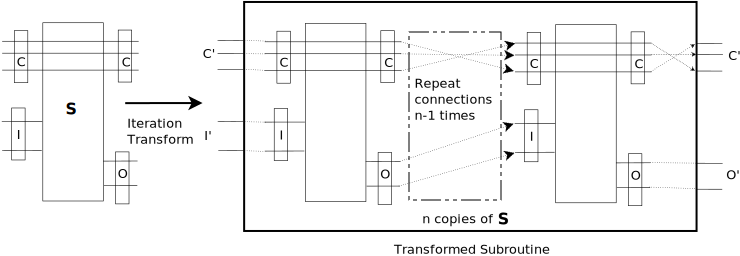
\includegraphics[scale=.4]{diagrams/SubroutineIterationTransform.png}
   \caption{Transforming a subroutine to an iterated subroutine}
   \label{fig:transforming_a_subroutine_to_an_iterated_subroutine}
\end{figure}
% subsection iteration_transformation_of_a_subroutine (end)

\subsection{Folding subroutines} % (fold)
\label{sub:folding_subroutines}

In addition to the concept of iteration the ability to fold subroutines over data structures could
also be useful. A folded call of a subroutine is similar to an iteration, in that controls and
possibly some of the inputs and outputs are iterated. The difference occurs in that we expect to
take some of the inputs from a data structure and return some of the outputs to a data structure.
An example of this would be folding over a list of \qubit{s} where each qubit is taken as a input
for each iteration.

First, we will examine the requirements for a non-linear safe fold, that is, where no input
duplication on the control wires is allow

\begin{definition}\label{def:linear_only_subroutine_fold}
  Given a subroutine $S=([gate],C,I,O,c,r,n)$, a starting context of typed wires $W_1$ and a data
  structure on wires $D\subset W_1$, a \emph{linear-only folded call} of $S$ over $D$ resulting in
  the context of typed wires $W_2$ and the data structure $E\subset W_2$ consists of the tuple
  $(CI_f,CO_f, g, h, ciof_b, s_{in}, s_{out})$ where
  \begin{itemize}
    \item $CI_f::\type{Arity}, \dom{CI_f} \subset \dom{C}\cup \dom{I}$,
    \item $CO_f::\type{Arity}, \dom{CO_f} \subset \dom{C}\cup \dom{O}$,
    \item $g:\dom{C}\cup\dom I / \dom{CI_f} \to W_1$ and $g$ is injective,
    \item $h:\dom{C}\cup\dom O /\dom{CO_f} \to W_2$ and $h$ is injective,
    \item $ciof_b$ is a bijection between the sets $(\dom{C}\,\cup\,\dom{O})/\dom{CO_f}$
      and $(\dom{C}\,\cup\,\dom{I})/\dom{CI_f}$,
    \item $s_{in}: \dom{CI_f} \to W_1$ (pulls from $D$),
    \item $s_{out}: \dom{CO_f} \to W_2$ (pushes to $E$),
    \item $g + s_{in} \in F(\nothing,I,W_1)$,
    \item $ciof_b^{-1} + s_{in} \in F(\nothing,I,W_1)$,
    \item $ciof_b + s_{out} \in F(\nothing,O,W_2)$,
    \item $h + s_{out} \in F(\nothing,O,W_2)$,
    \item $|\dom{CI_f}| = leafsize(D)$,
    \item $leafsize(E) = |\dom{CO_f}|$.
  \end{itemize}
\end{definition}

\begin{definition}\label{def:structured_linear_folded_call}
  Given the data for an linear-only folded call, a \emph{structured linear-only folded call} is a
  pair of high level structures $(i_s,o_s)$ and $(i_{fs},o_{fs})$ and a pair of quantum terms
  $(a,b)$ such that:
  \begin{itemize}
    \item $i_s(a) = g + s_{in}$,
    \item $o_s(h + s_{out}) = b$,
    \item $i_{fs}(a) = s_{in}$, and
    \item $o_{fs}(s_{out}) = b$.
  \end{itemize}

\end{definition}

Discussion points:
\begin{itemize}
  \item Does the structured call get rid of the last two items regarding leafsize? Same issue with
  non-linear safe call.
  \item For the structured call, it appears to me that there is only one pair of terms $a,b$ with
  two different (de)structuring morphisms.
\end{itemize}

The action on the wires of the calling program will be given by this relation:
\[
  s_{out} + h \circ (s_{out} + cio_f + s_{in})^{len(D)} \circ (g + s_{in})^{-1}.
\]
\begin{example}[Fold over Carry]\label{ex:fold_over_carry}

  For this example, we use the carry portion of the addition algorithm found in
  \cite{Vedral:1995ga}.

  The carry circuit is shown below:
  \[
    \Qcircuit @C=1em @R=.7em {
      \lstick{anc} & \ctrl{2} & \qw & \qw & \rstick{anc} \qw \\
      \lstick{a}  & \qw & \ctrl{1} & \ctrl{1} & \rstick{a} \qw \\
      \lstick{b}  & \ctrl{1} & \targ & \ctrl{1} & \rstick{b} \qw \\
      \lstick{c}  & \targ & \qw& \targ & \rstick{c} \qw
    }
  \]

  The intent of this circuit is to compute the final carry when adding the quregisters $A$ and $B$.
  The input prepares the $anc$ in state $\ket{0}$ and an auxiliary register $R$, the same size as
  $A$ and $B$ as $\ket{00\ldots0}$. Assume that $A = [w_1,w_2,w_3], B=[w_4,w_5,w_6], anc=w_7$ and
  $R=[w_8,w_9,w_{10}]$. $(A,B,R)$, a tuple of three registers forms our $D$ --- the input to the
  fold. Then, we may perform a folded call of carry as follows:
  \begin{itemize}
    \item $\dom{C} = \{anc,a\},\ \dom{I} = \{b,c\} = \dom{O}$;
    \item $\dom{CI_f} = \{a,b,c\}$ and $\dom{CO_f} = \{anc,a,b\}$;
    \item $g = \{anc \mapsto w_{6}\}$, $h=\{c\mapsto w_{10}\}$
    \item $ciof_b = \{c \mapsto anc \}$
    \item $s_{in} = \{a \mapsto D[0], b \mapsto D[1], c \mapsto D[2]\}$
    \item $s_{out} = \{anc \mapsto E[2], a \mapsto E[0], b \mapsto E[1]\}$.
  \end{itemize}
  From the mapping $s_{out}$, we set $E = (A,B,R')$ where $R'=[w_7,w_8,w_9]$.
\end{example}

Discussion points:
\begin{itemize}
  \item Is there a non-linear safe use case? Carry seemed quite simple,
    but it required linear safe inputs when folded.
  \item Each fold iteration input might be multiple \qubit{s},
    combined into a single data structure, as in 
    \vref{ex:fold_over_carry}.
  \item The number of inputs and outputs no longer need
    to agree as they did in iteration.  An example would be a subroutine that
    applied a two \qubit gate and then discarded one of the \qubits.
    The fold would be expected to convert a list of pairs  of \qubit{s}
    to a list of \qubit{s}. (Note this subroutine would not be reversible
    or controllable).
  \item The shape of the foldable in and out as well as the number of \qubits
    at each leaf would need to be known.
  \item The $F(C,K,W)$ permissible functions are not quite right for
    linear-only folds --- we do not want to allow duplication of any of
    the inputs, so rather than $F(C,K,W)$ we must use $F(\nothing,C+K,W)$.
\end{itemize}

\begin{definition}\label{def:subroutine_fold}
  Given a subroutine $S=([gate],C,I,O,c,r,n)$, a starting context of typed wires $W_1$ and a data
  structure on wires $D\subset W_1$, a \emph{folded call} of $S$ over $D$ resulting in the context
  of typed wires $W_2$ and the data structure $E\subset W_2$ consists of the tuple $(I_f,O_f,
  f_{in}, f_{out}, g, h, c_b, iof_b, s_{in}, s_{out} )$ where
  \begin{itemize}
    \item $I_f::\type{Arity}, \dom{I_f} \subset \dom{I}$,
    \item $O_f::\type{Arity}, \dom{O_f} \subset \dom{O}$,
    \item $f_{in}:\dom C \to W_1\cup W_2$
    \item $f_{out}:\dom C \to W_1\cup W_2$
    \item $g:\dom I / \dom{I_f} \to W_1$
    \item $h:\dom O /\dom{O_f} \to W_2$
    \item $c_b$ is a bijection (permutation) of $C$,
    \item $iof_b$ is a bijection between $\dom{O}/\dom{O_f}$ and $\dom{I}/\dom{I_f}$,
    \item $s_{in}: \dom{I_f} \to W_1$ (pulls from $D$)
    \item $s_{out}: \dom{O_f} \to W_2$ (pushes to $E$)
    \item $f_{in}+ g+ s_{in} \in F(C,I,W_1)$,
    \item $f_{out}+ h + s_{out} \in F(C,O,W_2)$,
    \item $iof_b + s_{in} \in F(\nothing,I,W_1)$,
    \item $iof_b + s_{out} \in F(\nothing,O,W_2)$,
    \item $|\dom{I_f}| = leafsize(D)$
    \item $leafsize(E) = |\dom{O_f}|$
  \end{itemize}

\end{definition}

\begin{definition}\label{def:structured_folded_call}
  Given the data for an folded call, a \emph{structured folded call} is a pair of high level
  structures $(i_s,o_s)$ and $(i_{fs},o_{fs})$ and a pair of quantum terms $(a,b)$ such that:
  \begin{itemize}
    \item $i_s(a) = f_{in}+g + s_{in}$,
    \item $o_s(f_{out} + h + s_{out}) = b$,
    \item $i_{fs}(a) = s_{in}$, and
    \item $o_{fs}(s_{out}) = b$.
  \end{itemize}
\end{definition}

% subsection folding_subroutines (end)

\subsection{Subroutine to folded subroutine transform} % (fold)
\label{sub:subroutine_to_folded_subroutine_transform}

In order to transform a given subroutine, we require the following data:
\begin{itemize}
  \item A bijection from some subset of the control and output wires to some subset of the control
    and input wires;
  \item a count of the number of iterations.
\end{itemize}

This allows us to derive a new $C,I,O$ for the fold subroutine. We proceed with the formal
definition.
\begin{definition}\label{def:fold_transform_of_a_subroutine}
  The \emph{fold transform} of a subroutine is a function $S_f$ with parameters $(n,b_{cio})$ which
  takes the subroutine $(g,C,I,O,r,c,n)$ to the subroutine $(g',C',I',O',r,c,n)$. The
  parameters have the following types:
  \begin{align*}
    n&::\type{Int}, n>0;\\
    b_{cio}&::\type{bijection(CI \leftrightarrow CO)} \\
    &\text{where }CI\subseteq C\cup I\text{ and }\subseteq C\cup O.
  \end{align*}
\end{definition}

Note that $b_{cio}$ may be defined as a set of ordered pairs
\begin{equation}
  \{(f,t)|f\in C\cup I, t \in C\cup O,\text{ and } f,t \text{ appear at most once}\}.
  \label{eq:defintion_of_bcio}
\end{equation}
The data we need to create for the end result are the set of control wires, the input and output
wires and the new gates sequence. We proceed with presenting the algorithm for the control wires.

When considering which inputs (and hence outputs) are control wires in the transformed subroutine,
we must follow the path of a control input. A control input to the base subroutine will remain a
control input to the transformed subroutine only if its full folded path contains only control
wires before exiting. Depending upon the structure of $b_{cio}$ it is possible all, none or some
finite subset of specific control wires become controls for the transformed routine.

To determine if a wire is a control, we will calculate a characteristic of the wire and show that
it requires at most $k$ iterations to calculate, where $k$ is the number of control wires of the
original subroutine.

First, define:
\begin{align*}
  \Omega &:: C \to C \cup \{*,@\}\\
  \Omega(c) &=
  \begin{cases}
    c'&\text{if }b_{cio}(c) = c'\text{ and }c'\in C,\\
    *&\text{if $c$ is not the first element of any pair in }b_{cio},\\
    @&\text{if }b_{cio}(c) = j\text{ and }j\in I.
  \end{cases}
\end{align*}
Then, noting that $k = |C|$, define:
\begin{align*}
  \Gamma &:: C \to \nat \cup \{\infty\}\\
  \Gamma(c) &=
  \begin{cases}
    \infty & \Omega(c) = *,\\
    0 & \Omega(c) = @,\\
    1 + \Gamma(\Omega(c)) & \Gamma(\Omega(c)) < k,\\
    \infty & \Gamma(\Omega(c)) \ge k.
  \end{cases}
\end{align*}

Dually, we may define functions  $\Theta(c)$ and $\Delta(c)$:
\begin{align*}
  \Theta &:: C \to C \cup \{*,@\}\\
  \Theta(c) &=
  \begin{cases}
    c'&\text{if }b_{cio}(c') = c\text{ and }c'\in C,\\
    *&\text{if $c$ is not the second element of any pair in }b_{cio},\\
    @&\text{if }b_{cio}(o) = c\text{ and }o\in O.
  \end{cases}\\
  \Delta &:: C \to \nat \cup \{\infty\}\\
  \Delta(c) &=
  \begin{cases}
    \infty & \Theta(c) = *,\\
    0 & \Theta(c) = @,\\
    1 + \Delta(\Theta(c)) & \Delta(\Theta(c)) < k,\\
    \infty & \Delta(\Theta(c)) \ge k.
  \end{cases}
\end{align*}

Note that in the case of cycles among control wires, the cycle \emph{must} be of size $k$ or less.
As such, at most $k$ iterations of $\Gamma$ are required before confirming a value for $\Gamma(c)$.
The same argument applies to computing $\Theta$.

Assuming that $C$ is ordered, the data for $b_{cio}$ may be stored such that computing $b_{cio}(c)$
and therefore $\Omega(c)$ is of $\BigO{\log k}$. Therefore, $\Gamma$ is of complexity $\BigO{k\log
k}$ and computing $\Gamma$ for all of $C$ will then be of $\BigO{k^2 \log k}$. Computing $\Delta$
will have the same complexity.

We may now describe the algorithm for determining control wires, $C'$ input wires, $I'$ and output
wires, $O'$ of the transformed subroutine. In the algorithm, $n$ is the number of iterations, $k$
is the cardinality of $C$. Additionally, we compute a \emph{rank} of each $c$ in $C'$. The
\emph{rank} of $c$ is the number of iterations that $c$ will go through.
\begin{enumerate}
  \item Add all members of $I$ to $I'$, subscripting with $1$.
  \item For all $i\in I$ where $i \nin \rng b_{cio}$, add $i_2,i_3,\ldots,i_n$ to $I'$.
  \item Add all members of $O$ to $O'$, subscripting with $n$.
  \item For all $o\in O$ where $o \nin \dom b_{cio}$, add $o_1,o_2,\ldots,o_{n-1}$ to $O'$.
  \item Partition $C$ into four subsets:
  \begin{align*}
    C_*    &= \{c|c\nin \dom b_{cio}\text{ and }c\nin \rng b_{cio}\},\\
    C_d    &= \{c|c\in \dom b_{cio}\text{ and }c\nin \rng b_{cio}\},\\
    C_r    &= \{c|c\nin \dom b_{cio}\text{ and }c\in \rng b_{cio}\},\\
    C_{dr} &= \{c|c\in \dom b_{cio}\text{ and }c\in \rng b_{cio}\}.
  \end{align*}
  \item For each $c\in C_*$, add $c_1,c_2,\ldots,c_n$ to $C'$. Set the
    rank of each of these to $0$.
  \item For each $c\in C_d$, compute $j=\Gamma(c)$. If $j \ge n$, add
    $c_1,c_2,\ldots,c_n$ to $C'$. If not, then:
    \begin{itemize}
      \item Add $c_{n-j},c_{n-j+1},\ldots,c_n$ to $C'$, setting the
        rank of $c_\ell$ to $n-\ell$.
      \item Add $c_1,c_2,\ldots,c_{n-j-1}$ to $I'$.
    \end{itemize}
  \item For each $c\in C_r$, compute $m=\Delta(c)$. If $m \ge n$, add
    $c_1,c_2,\ldots,c_n$ to $C'$, setting each item to rank $0$.
    If not, then:
    \begin{itemize}
      \item Add $c_1,c_2,\ldots,c_{j+1}$ to $C'$, setting each rank to $0$.
      \item Add $c_{j+2},c_{j+3},\ldots,c_{n}$ to $I'$.
    \end{itemize}
  \item For each $c\in C_{dr}$, compute $j=\Gamma(c), m=\Delta(c)$. Then
    if $j>n-1$, add $c_1$ to $C'$, setting its rank to $n-1$, otherwise
    add it to $I'$. Conversely, if $m>n-1$, add $c_n$ to $C'$, setting its
    rank to $0$, otherwise add it to $O'$. In the case
    where both $c_1$ and $c_n$ are added to $C'$, we have actually added
    one too many items to $C'$ as there will be a duplication. This is
    addressed in the final step, where the in-out names of the control
    wires are reconciled.
  \item Reconcile the $C'$ names: For each $c_h\in C'$, compute
    $x=b_{cio}^{Rank(c)}(c)$. In $C'$, replace $x_n$ with $c_h$. After
    completing this computation, remove any duplicates.
\end{enumerate}

% The above algorithm will compute the correct $C'$ and $I'$ for the transformed
% subroutine. Additionally, we must also compute the matching of the control
% wires on input and output. To do this, we must essentially trace the path
% of each of the wires in $C'$ and determine what is the final output. There
% are three cases to consider for each $c$:
% \begin{itemize}
%   \item $\Gamma(c_m) = j>0$. This means that $c_m$ is an input with $j$ or
%     fewer iterations remaining. Compute $c' = \Omega^{rank(c_m)}(c)$. The name
%     matched with $c_m$ is then $c'_{m+rank(c_m)}$.
%   \item $\Gamma(c) = \infty, \Omega(c)=*$. $c$ is an immediate in/out control
%     wire.
%   \item $\Gamma(c) = \infty, \Omega(c)=c'$. This case occurs when $c$ is part
%     of a cycle. As noted above, the cycle must be of length $j \le k$. Hence,
%     compute $c_{\ell}=\Omega^{\ell}(c)$ where $\ell=n-1 \mod j$. Then
%     $c_\ell$ is the name of the output matched with $c$.
% \end{itemize}


% subsection subroutine_to_folded_subroutine_transform (end)
\subsection{Examples of folding} % (fold)
\label{sub:examples_of_folding}

\begin{example}\label{exmpl:fold_example_with_three_mixed_in_out}
  Consider $S=(\_,\{a,b\},\{c\},\{d\},\_,\_,\_)$ and $b_{cio}=\{(a,c),(b,a)\}$ and an iteration
  count of $3$. See \vref{fig:Fold_with_extra_in_out}.
\end{example}
\begin{figure}[htbp]
  \centering
    \[
      \Qcircuit{
       & \dqw& \dqw &\dqw &\dqw &\dqw\ar@{.} [dddr]&\\
       & \dqw& \dqw\ar@{.}[ddr]\\
       & \multigate{3}{S_1}_{a_1} & \qw  \ar@{.}[dddr] &  & \multigate{3}{S_2}_{a_2}&\qw\ar@{.}[dddr]&  & \multigate{3}{S_3}_{a_3}&\qw\\
       & \ghost{S_1}_{b_1} & \qw \ar@{.}[ur]& &\ghost{S_2}_{b_2}&\qw\ar@{.}[ur]& &\ghost{S_3}_{b_3}&\qw\\
       &  & & & & & & & & & &\\
       & \ghost{S_1}_{c_1}& \qw_{d_1} \ar@{.}[ddr]& &\ghost{S_2}_{c_2}&\qw_{d_2}\ar@{.}[dr]& &\ghost{S_3}_{c_3}&\qw_{d_3}\\
       &            &                & &            &              & &\dqw&\dqw\\
       &            &                & & \dqw      &\dqw           &\dqw&\dqw&\dqw
      }
    \]
  \caption{Fold with extra in/out}
  \label{fig:Fold_with_extra_in_out}
\end{figure}

From the data, we compute:
\begin{align*}
  \Omega(a) &= @\text{ and }\Omega(b) = a,\\
  \Gamma(a) &=0\text{ and }\Gamma(b) = 1,\\
  \Theta(b) &=*\text{ and }\Delta(b)=\infty,\\
  \Theta(a)=b\text{ and } \Delta(a)=\infty.
\end{align*}

Now, following the steps of the algorithm,
\begin{enumerate}
  \item $I' \mapsto \{c_1\}$.
  \item No change to $I'$.
  \item $O' \mapsto \{d_3\}$.
  \item $O' \mapsto \{d_1,d_2,d_3\}$.
  \item $C_*=\nothing, C_d=\{b\}, C_r =\nothing, C_{dr}=\{a\}$.
  \item For $C_d$, As $\Gamma(b)=1$, we have $C' \mapsto \{b_2,b_3\}$ and
    $I' \mapsto \{c_1,b_1\}$. The rank of $b_2$ is 1 and the rank of $b_3$
    is 0.
  \item For $C_{dr}=\{a\}$, $\Gamma(a)=0$ and $\Delta(a)=\infty$, therefore
    we add $a_1$ to $I'$ and $a_3$ to $C'$. The rank of $a_3$ is zero.
    At this stage, we now have
    $I'=\{c_1,b_1,a_1\}, O'=\{d_1,d_2,d_3\}$ and $C'=\{b_2,b_3,a_3\}$.
  \item Reconcile $C'$: $b_{cio}(b)=a$ and $b_{cio}(a)=c$, therefore
    $b_{cio}^1(b_2)=a_3$, $b_{cio}^0(b_3)=b_3$, and $b_{cio}^0(a_3)=a_3$.
    Following our replacement scheme, $C'=\{b_2,b_3\}$.
\end{enumerate}

Hence our final result is:
\begin{align*}
  I'&=\{c_1,b_1,a_1\},\\
  O'&=\{d_1,d_2,d_3\}\text{ and}\\
  C'&=\{b_2,b_3\}.
\end{align*}

\begin{example}\label{exmpl:fold_example_with_partial_bcio}
  Consider $S=(\_,\{a,b\},\{c\},\{d\},\_,\_,\_)$ as in 
  \vref{exmpl:fold_example_with_three_mixed_in_out} and
  $b_{cio}=\{(a,c),(b,a),(d,b)\}$ and an iteration count of $3$. See 
  \vref{fig:Fold_with_three_iterations}.
\end{example}
\begin{figure}[htbp]
  \centering
  \[
    \Qcircuit{
     & \multigate{3}{S_1}_{a_1} & \qw  \ar@{.}[dddr] &  & \multigate{3}{S_2}_{a_2}&\qw\ar@{.}[dddr]&  & \multigate{3}{S_3}_{a_3}&\qw\\
     & \ghost{S_1}_{b_1} & \qw \ar@{.}[ur]& &\ghost{S_2}_{b_2}&\qw\ar@{.}[ur]& &\ghost{S_3}_{b_3}&\qw\\
     &  & & & & & & & & & &\\
     & \ghost{S_1}_{c_1}& \qw_{d_1} \ar@{.}[uur]& &\ghost{S_2}_{c_2}&\qw_{d_2}\ar@{.}[uur]& &\ghost{S_3}_{c_3}&\qw_{d_3}\\
    }
  \]
  \caption{Fold with three iterations}
  \label{fig:Fold_with_three_iterations}
\end{figure}

From the data, we have:
\begin{align*}
  \Omega(a) &= @\text{ and }&\Gamma(a)=0,\\
  \Omega(b) &= a\text{ and }&\Gamma(b) = 1,\\
  \Theta(b)&=@\text{ and }&\Delta(b)=0,\\
  \Theta(a)&=b\text{ and }&\Delta(a)=1.
\end{align*}

Now, following the steps of the algorithm,
\begin{enumerate}
  \item $I' \mapsto \{c_1\}$.
  \item No change to $I'$.
  \item $O' \mapsto \{d_3\}$.
  \item All $o$ are in the range of $b_{cio}$, therefore no further
    change to $O'$.
  \item $C_*=C_d=C_r = \nothing, C_{dr}=\{a,b\}$.
  \item As $n-1=2 > \Gamma(a),\Gamma(b)$, we have $I'
    \mapsto \{c_1,a_1,b_1\}$. Similarly, since $n-1=2 > \Delta(a),\Delta(b)$,
    $O'\mapsto \{a_3,b_3,d_3\}$
  \item With $C'$ empty, there are no further steps.
\end{enumerate}
Hence our final result is:
\begin{align*}
  I'&=\{c_1,b_1,a_1\},\\
  O'&=\{a_3,b_3,d_3\}\text{ and}\\
  C'&=\nothing.
\end{align*}

\begin{example}\label{exmpl:fold_transform_example_of_carry}
  Consider $C=(\_,\{r,a\},\{b,c\},\{d,e\},\_,\_,\_)$,
  $b_{cio}=\{(e,r)\}$ and an iteration count of $4$. See 
  \vref{fig:fold_carry_transformed}.
\end{example}
\begin{figure}[htbp]
  \centering
  \[
    \xymatrix @R=7pt @*=<0em>{
     & \multigate{3}{C}_{r_1} & \qw& \qw & \qw & \qw & \qw & \qw & \qw\\
     & \ghost{C}_{a_1} & \qw       & \qw & \qw & \qw & \qw & \qw & \qw\\
     & \ghost{C}_{b_1} & \qw_{d_1} & \qw & \qw & \qw & \qw & \qw & \qw\\
     & \ghost{C}_{c_1} & \qw_{e_1} & \multigate{3}{C}_{r_2} & \qw & \qw & \qw & \qw  & \qw\\
     & \qw_{a_2}       & \qw       & \ghost{C} & \qw        & \qw & \qw & \qw & \qw\\
     & \qw_{b_2}       & \qw       & \ghost{C} & \qw_{d_2}  & \qw & \qw & \qw & \qw \\
     & \qw_{c_2}       & \qw       & \ghost{C} & \qw_{e_2}  & \multigate{3}{C}_{r_3} &\qw& \qw & \qw\\
     & \qw_{a_3}       & \qw       & \qw       & \qw        & \ghost{C} &\qw      & \qw & \qw \\
     & \qw_{b_3}       & \qw       & \qw       & \qw        & \ghost{C} &\qw_{d_3}& \qw & \qw\\
     & \qw_{c_3}       & \qw       & \qw       & \qw        & \ghost{C} &\qw_{e_3}& \multigate{3}{C}_{r_4} &\qw\\
     & \qw_{a_4}       & \qw       & \qw       & \qw        & \qw       & \qw     & \ghost{C} &\qw\\
     & \qw_{b_4}       & \qw       & \qw       & \qw        & \qw       & \qw     & \ghost{C} &\qw_{d_4}\\
     & \qw_{c_4}       & \qw       & \qw       & \qw        & \qw       & \qw     & \ghost{C} &\qw_{e_4}\\
    }
  \]
  \caption{Fold of Carry}
  \label{fig:fold_carry_transformed}
\end{figure}

From the data, we have:
\begin{align*}
  \Omega(r) &= *\text{ and }&\Omega(a) = *,\\
  \Gamma(r)&=\infty\text{ and }&\Gamma(a) = \infty,\\
  \Theta(r)&=@\text{ and }&\Delta(r)=0,\\
  \Theta(a)=*\text{ and } &\Delta(a)=\infty.
\end{align*}

Now, following the steps of the algorithm,
\begin{enumerate}
  \item $I' \mapsto \{b_1,c_1\}$.
  \item No element of $I$ is in $b_{cio}$, therefore we have
    $I' \mapsto \{b_1,c_1,b_2,c_2,b_3,c_3,b_4,c_4\}$
  \item $O' \mapsto \{d_4,e_4\}$.
  \item Only $e$ is in the range of $b_{cio}$, therefore we add
    $d_1,d_2,d_3$ to  $O'$, giving us $\{d_1,d_2,d_3,d_4,e_4\}$.
  \item $C_*=\{a\},C_d=\nothing, C_r = \{r\},\ C_{dr}=\nothing$.
  \item Considering $C_*$, we add $\{a_1,a_2,a_3,a_4\}$ to $C'$, each with rank 0.
  \item Next considering $C_r$, as $\Delta(r)=0$, we add $r_1$ to $C'$ with
    rank 0 and then add $r_2,r_3,r_4$ to $O'$.
  \item As each element of $C'$ is of rank 0, there is no changes to the names.
\end{enumerate}

Hence our final result is:
\begin{align*}
  I'&=\{b_1,c_1,b_2,c_2,b_3,c_3,b_4,c_4\},\\
  O'&=\{d_1,d_2,d_3,d_4,e_4,r_2,r_3,r_4\}\text{ and}\\
  C'&=\{r_1,a_1,a_2,a_3,a_4\}.
\end{align*}

% subsection examples_of_folding (end)
% section subroutine_calls_and_transformers (end)

% section diagram_of_folded_carry (end)
\section{Alternate Algorithm for Fold Transformation} % (fold)
\label{sec:alternate_algorithm_for_fold_transformation}
In this section, we present an alternate algorithm for calculating the type and names of control,
input and output wires for a folded subroutine. The starting point is
\vref{def:fold_transform_of_a_subroutine} and the ordered pairs of $b_{cio}$: A set of ordered
pairs $\{(f,t)|f\in C\cup I, t \in C\cup O\}$.

To implement the algorithm of calculating the folded subroutines $C,I$ and $O$, we need the
following:
\begin{itemize}
  \item $I\cap O = \nothing$, which may be accomplished by renaming if needed.
  \item We create the sets $C_j,I_j,O_j$ for $j=1\ldots n$ where the members
    of $X_j$ are the elements of $X$ together with the subscript $j$ where
    $X$ is one of $C,I,O$.
\end{itemize}

The algorithm proceeds by creating a set of ``type'' constraints for each of the elements of the
new sets, based upon $b_{cio}$ and membership in a $C,I$ or $O$ set.

The algorithm steps are:
\begin{enumerate}
  \item Create a set $\mathcal{C}$ of pairs $(a_j,b_{j+1})$ for $j$
  ranging from $0$ to $n-1$ based upon the bijection $b_{cio}$.
  \item For each $j=0\ldots n-1$,
  \begin{enumerate}
    \item For all $c\in C_j$, if $(c,\_)\notin\mathcal{C}$,
      add the pair $(c,\nothing)$
    \item For all $c\in C_j$, if $(\_,c)\notin\mathcal{C}$,
      add the pair $(\nothing,c)$
    \item For all $o\in O_j$, if $(o,\_)\notin\mathcal{C}$,
      add the pair $(o,\nothing)$
    \item For all $i\in I_j$, if $(\_,i)\notin\mathcal{C}$,
      add the pair $(\nothing,i)$
  \end{enumerate}
  \item Convert the pairs in $\mathcal{C}$ to equations and constraints as
    follows for each pair $(a,b)$:
  \begin{enumerate}
    \item $a=\nothing\implies \begin{cases}
      b::(b,C)&\text{when }b\in C_j\text{for some }j,\\
      b::(b,I)&\text{when }b\in I_j\text{for some }j.
    \end{cases}$
    \item $a\in C_{j-1}\implies \begin{cases}
      b=a&\text{when }b\in C_j,\\
      b=a, b::I&\text{when }b\in I_j,\\
      a::(C,a)&\text{when }b=\nothing.
    \end{cases}$
    \item $a\in O_{j-1}\implies \begin{cases}
      b=a, b::O&\text{when }b\in C_j,\\
      \text{no equation}&\text{when }b\in I_j,\\
      a::(O,a)&\text{when }b=\nothing.
    \end{cases}$
  \end{enumerate}
  \item Solve the equations with the constraints, with the assumption that
    \[\xymatrix{
      &C\ar[dl]\ar[dr] \ar[d] & \\
      I \ar[dd]&(C,b)\ar[dr] \ar[d]&O\ar[d] \\
      &(b,C)\ar[dl]& (O,b) \\
      (b,I)& & }
    \]
  For example,
  \begin{itemize}
    \item $a::O, a::C$ is solvable with $a::O$;
    \item $a=b,b::(b,C),a::I$ is solved by $b,a::(b,I)$;
    \item $a=b, b=d, a::(a,C), d::(C,d)$ is solved by $a,b,d::(a,C)$.
  \end{itemize}
  \item For the folded subroutine, $X$ will be all items of ``type'' $X$,
    where $X$ is any of $C,I,O$, the names of each entry will be the companion
    name with the ``type''.
\end{enumerate}
\note{The algorithm above works correctly, but likely has too high of a complexity, depending on
the number of iterations. Need to revise in the next version to see if we can make the complexity
proportional to the number of wires in/out.}

\subsection{Examples of folding with Alternate Algorithm} % (fold)
\label{sub:examples_of_folding_with_alternate_algorithm}
\begin{example}\label{exmpl:alternate_fold_example_with_three_mixed_in_out}
  We repeat \vref{exmpl:fold_example_with_three_mixed_in_out}, that is,
  $S=(\_,\{a,b\},\{c\},\{d\},\_,\_,\_)$ and $b_{cio}=\{(a,c),(b,a),(d,b)\}$
  and an iteration count of $3$. See \vref{fig:Fold_with_three_iterations}.
\end{example}
There are two control wires $a,b$, an input wire $d$ and one output wire $d$. We will do three
iterations. Our set $\mathcal{C}$ of pairs becomes:
\begin{align*}
  \{ & (\nothing,a),\ (\nothing,b),\ (\nothing,c),\\
  & (b,a_1),\ (d,b_1),\ (a,c_1),\\
  & (b_1,a_2),\ (d_1,b_2),\ (a_1,c_2),\\
  & (a_2,\nothing),\ (b_2,\nothing),\ (c_2,\nothing)\}.\\
\end{align*}
Translating each of these to equations and constraints, we get:
\begin{align*}
  &a::(a,C), b::(b,C), c::(c,I)\\
  &b=a_1, b_1=d\ b_1::O, a=c_1\ c_1::I\\
  &b_1=a_2, b_2=d_1\ b_2::O, a_1=c_2\ c_2::I\\
  &a_2::(C,a_2), b_2::(C,b_2), d_2::(O,d_2)
\end{align*}
As we have three wires in and three wires out, we expect to see six separate
groupings in the solution to the above equations. We will proceed by starting
from the top left.
\begin{align*}
  \text{start: }a &\quad a=c_1, ::I, ::(a,C) &\implies a::(a,I)\\
  \text{start: }b &\quad  b=a_1,a_1=c_2, ::I, ::(b,C) &\implies b::(b,I)\\
  \text{start: }c &\quad  ::(c,I) &\implies c::(c,I)\\
  \text{start: }b_1 &\quad  b_1=d, b_1=a_2, ::O, ::(C,a_2) &\implies
    a_2::(O,a_2)\\
  \text{start: }b_2 &\quad  b_2=d_1, ::O, ::(C,b_2) &\implies b_2::(O,b_2)\\
  \text{start: }d_2 &\quad  ::(O,d_2) &\implies d_2::(O,d_2)
\end{align*}
% subsection examples_of_folding (end)
% section alternate_algorithm_for_fold_transformation (end)



\begin{singlespace}
\bibliography{bibentries-phd}
\bibliographystyle{plain}
\end{singlespace}
\appendix
%%!TEX root = /Users/gilesb/UofC/thesis/phd-thesis/phd-thesis.tex
%\fancyhead[RO,LE]{\thepage}
%\fancyfoot{}

\chapter{First Appendix}

\begin{figure}
%   \centering
% 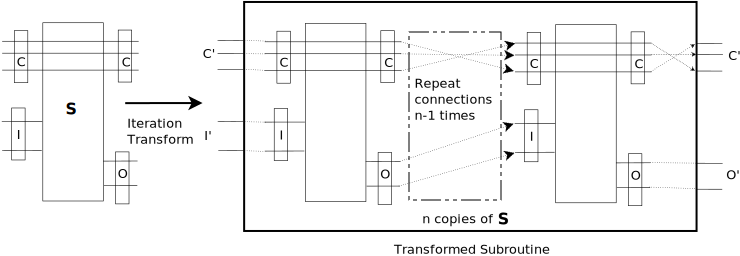
\includegraphics[scale=.4]{diagrams/SubroutineIterationTransform.png}
% \caption{Transforming a subroutine to an iterated subroutine}
% \label{fig:transforming_a_subroutine_to_an_iterated_subroutine}
\end{figure}


\end{document}
